\subsection{Sự ra đời và tầm quan trọng của mạng LSTM}
Như đã phân tích ở chương trước, mạng RNN truyền thống gặp phải vấn đề nghiêm trọng về việc tiêu biến đạo hàm (Vanishing Gradient), khiến nó không thể ghi nhớ các thông tin trong một khoảng thời gian dài. Để khắc phục nhược điểm này, năm \textbf{1997}, Sepp Hochreiter và Jürgen Schmidhuber đã đề xuất kiến trúc \textbf{Long Short-Term Memory (LSTM)}. 

LSTM nhanh chóng trở thành một cuộc cách mạng trong lĩnh vực học sâu. Với khả năng lưu trữ thông tin qua hàng trăm bước thời gian, LSTM đã trở thành nền tảng cho các hệ thống dịch thuật tự động (Google Translate), nhận dạng giọng nói (Siri, Alexa) và đặc biệt là dự báo các biến động phức tạp trong kinh tế và kỹ thuật.

\subsection{Cấu trúc và cơ chế Cổng (Gates) của LSTM}
Khác với RNN chỉ có một cấu trúc đơn giản bên trong đơn vị lặp lại, LSTM sở hữu một kiến trúc tinh vi hơn nhiều với sự xuất hiện của \textbf{Cell State} và các \textbf{Cổng (Gates)}.

\subsubsection{Cell State (Trạng thái ô)}
Cell State có thể được hình dung như một "băng chuyền" thông tin chạy xuyên suốt toàn bộ chuỗi dữ liệu. Thông tin trên băng chuyền này rất ít bị thay đổi, giúp nó có thể truyền tải các thông tin quan trọng từ quá khứ xa xôi đến hiện tại mà không bị suy giảm đáng kể.

\subsubsection{Cơ chế các Cổng điều khiển}
LSTM sử dụng 3 loại cổng để điều chỉnh luồng thông tin ra vào Cell State:
\begin{itemize}
    \item \textbf{Forget Gate (Cổng quên):} Quyết định thông tin nào từ Cell State cũ sẽ bị xóa bỏ.
    \item \textbf{Input Gate (Cổng vào):} Quyết định thông tin mới nào sẽ được cập nhật vào Cell State.
    \item \textbf{Output Gate (Cổng ra):} Quyết định phần thông tin nào từ Cell State sẽ được đưa ra làm đầu ra và trạng thái ẩn mới.
\end{itemize}

\subsection{Công thức toán học của LSTM}
Tại mỗi bước thời gian $t$, quá trình tính toán trong một đơn vị LSTM được thực hiện qua các bước sau:

\begin{enumerate}
    \item \textbf{Cổng quên (Forget Gate):} Quyết định thông tin cũ cần xóa bỏ.
    \begin{equation}
        f_t = \sigma(W_f \cdot [h_{t-1}, x_t] + b_f)
    \end{equation}
    
    \item \textbf{Cổng vào (Input Gate):} Quyết định thông tin mới cần lưu trữ.
    \begin{equation}
        i_t = \sigma(W_i \cdot [h_{t-1}, x_t] + b_i)
    \end{equation}
    \begin{equation}
        \tilde{C}_t = \tanh(W_C \cdot [h_{t-1}, x_t] + b_C)
    \end{equation}
    
    \item \textbf{Cập nhật Trạng thái ô (Update Cell State):}
    \begin{equation}
        C_t = f_t * C_{t-1} + i_t * \tilde{C}_t
    \end{equation}
    
    \item \textbf{Cổng ra (Output Gate):} Xác định giá trị đầu ra.
    \begin{equation}
        o_t = \sigma(W_o \cdot [h_{t-1}, x_t] + b_o)
    \end{equation}
    \begin{equation}
        h_t = o_t * \tanh(C_t)
    \end{equation}
\end{enumerate}

\subsubsection{Các biến thể của LSTM}
\begin{itemize}
    \item \textbf{Peephole LSTM:} Cho phép các cổng nhìn thấy Cell State trực tiếp.
    \item \textbf{GRU (Gated Recurrent Unit):} Phiên bản đơn giản hóa với ít tham số hơn.
    \item \textbf{Bidirectional LSTM:} Xử lý chuỗi theo cả hai hướng (quá khứ và tương lai).
    \item \textbf{Stacked LSTM:} Ghép nhiều lớp LSTM để tăng độ sâu của mô hình.
\end{itemize}

\subsubsection{Ưu điểm của LSTM so với RNN}
\begin{itemize}
    \item \textbf{Khắc phục Vanishing Gradient:} Các cổng cho phép thông tin lưu trữ lâu dài.
    \item \textbf{Selective Memory:} Có thể học được thông tin nào quan trọng để giữ lại.
    \item \textbf{Stable Training:} Gradient được kiểm soát tốt hơn, ít bị explode.
\end{itemize}

\subsubsection{Các ứng dụng thực tế của LSTM}
\begin{itemize}
    \item \textbf{Xử lý ngôn ngữ tự nhiên:} Machine Translation, Sentiment Analysis, Text Generation.
    \item \textbf{Dự báo thời gian:} Stock Price Prediction, Weather Forecasting, Traffic Prediction.
    \item \textbf{Computer Vision:} Action Recognition, Video Captioning.
    \item \textbf{Y học:} ECG Analysis, Disease Prediction from Time Series.
\end{itemize}

\subsubsection{Huấn luyện và tối ưu hóa LSTM}
\begin{itemize}
    \item \textbf{Data Preparation:} Sequence creation, normalization, train/validation split.
    \item \textbf{Architecture Design:} Number of layers, hidden units, dropout rates.
    \item \textbf{Training Tricks:} Gradient clipping, learning rate scheduling, early stopping.
    \item \textbf{Evaluation:} Time series cross-validation, metrics like RMSE, MAE.
\end{itemize}

\subsection{Thực nghiệm theo từng tập dữ liệu}

Trong chương này, chúng ta sẽ kiểm chứng sức mạnh của LSTM thông qua hai bài toán dự báo chuỗi thời gian phức tạp: Dự báo giá cổ phiếu (Google Stock) và Dự báo thời tiết.

Khởi tạo môi trường với các thư viện hỗ trợ xử lý dữ liệu chuỗi và mô hình LSTM.

\begin{figure}[H]
    \centering
    
\includegraphics[width=0.9\textwidth]{../code/ch4_lstm/images/1.png}
    \caption{Thiết lập các công cụ Deep Learning và thư viện Scikit-learn để chuẩn hóa dữ liệu đầu vào cho LSTM.}
\end{figure}

\textbf{Giải thích chi tiết:} Thiết lập này kết hợp TensorFlow/Keras cho mô hình LSTM và Scikit-learn để chuẩn hóa input. Preprocessing đúng cách rất quan trọng với dữ liệu chuỗi vì các giá trị khác scale có thể ảnh hưởng mạnh tới gradient và hội tụ.

\subsubsection{Bài toán 1: Dự báo giá cổ phiếu Google}
Dự báo tài chính là bài toán thách thức do dữ liệu có tính biến động cao và chịu ảnh hưởng của nhiều yếu tố phi tuyến tính.

\begin{figure}[H]
    \centering
    
\includegraphics[width=0.9\textwidth]{../code/ch4_lstm/images/2.png}
    \caption{Sinh dữ liệu giá cổ phiếu giả lập: Kết hợp các thành phần xu hướng (trend) và biến động ngẫu nhiên để tạo ra chuỗi dữ liệu thực tế.}
\end{figure}

\textbf{Giải thích chi tiết:} Dữ liệu tổng hợp này mô phỏng đặc điểm của giá cổ phiếu thực tế: một trend dài hạn cộng với nhiễu ngắn hạn. Nó giúp kiểm tra khả năng LSTM học được các pattern phi tuyến và tính biến động.

\begin{figure}[H]
    \centering
    
\includegraphics[width=0.9\textwidth]{../code/ch4_lstm/images/3.png}
    \caption{Mã nguồn thực hiện EDA cho dữ liệu tài chính: Phân tích xu hướng dài hạn và các chỉ số thống kê biến động.}
\end{figure}

\textbf{Giải thích chi tiết:} EDA tài chính cung cấp cái nhìn về tính stationarity, volatility và trend. Những phân tích này xác định cách chuẩn bị dữ liệu và cấu trúc mô hình LSTM phù hợp.

Kết quả phân tích đặc trưng giá cổ phiếu:

\begin{figure}[H]
    \centering
    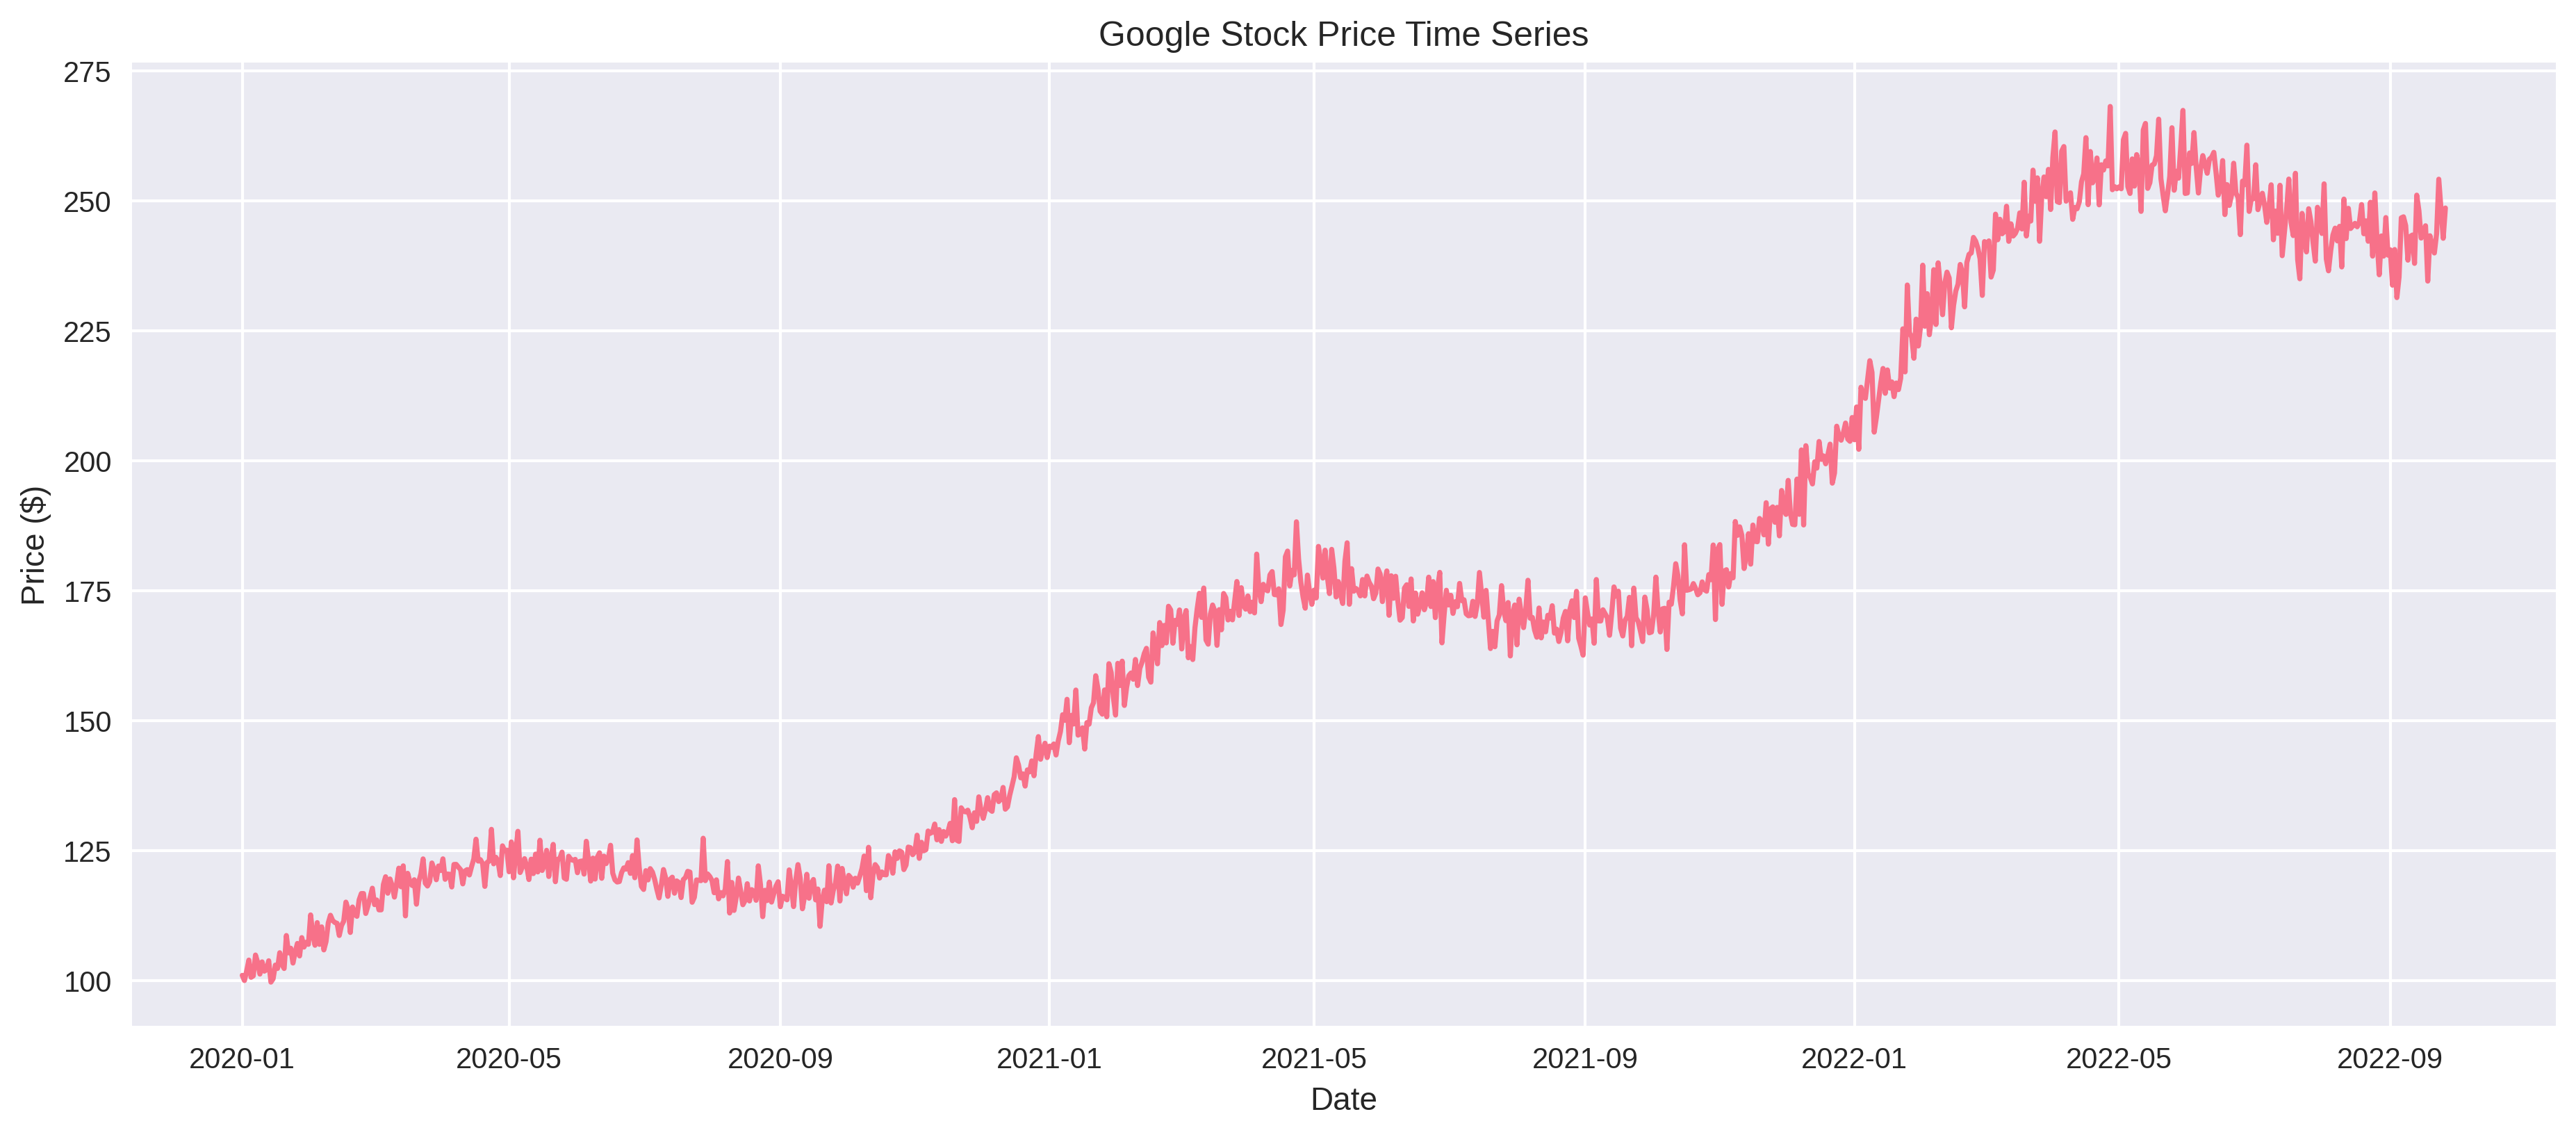
\includegraphics[width=0.75\textwidth]{../code/ch4_lstm/plots/google_stock_time_series.png}
    \caption{Chuỗi thời gian giá cổ phiếu: Trực quan hóa biến động giá trong một khoảng thời gian dài, xác định xu hướng tăng trưởng tổng thể.}
\end{figure}

\textbf{Giải thích chi tiết:} Visualization giúp nhận thấy trend tăng tổng thể và các dao động ngắn hạn. LSTM cần học cả hai yếu tố để dự báo chính xác, đặc biệt với dữ liệu tài chính có noise cao.

\begin{figure}[H]
    \centering
    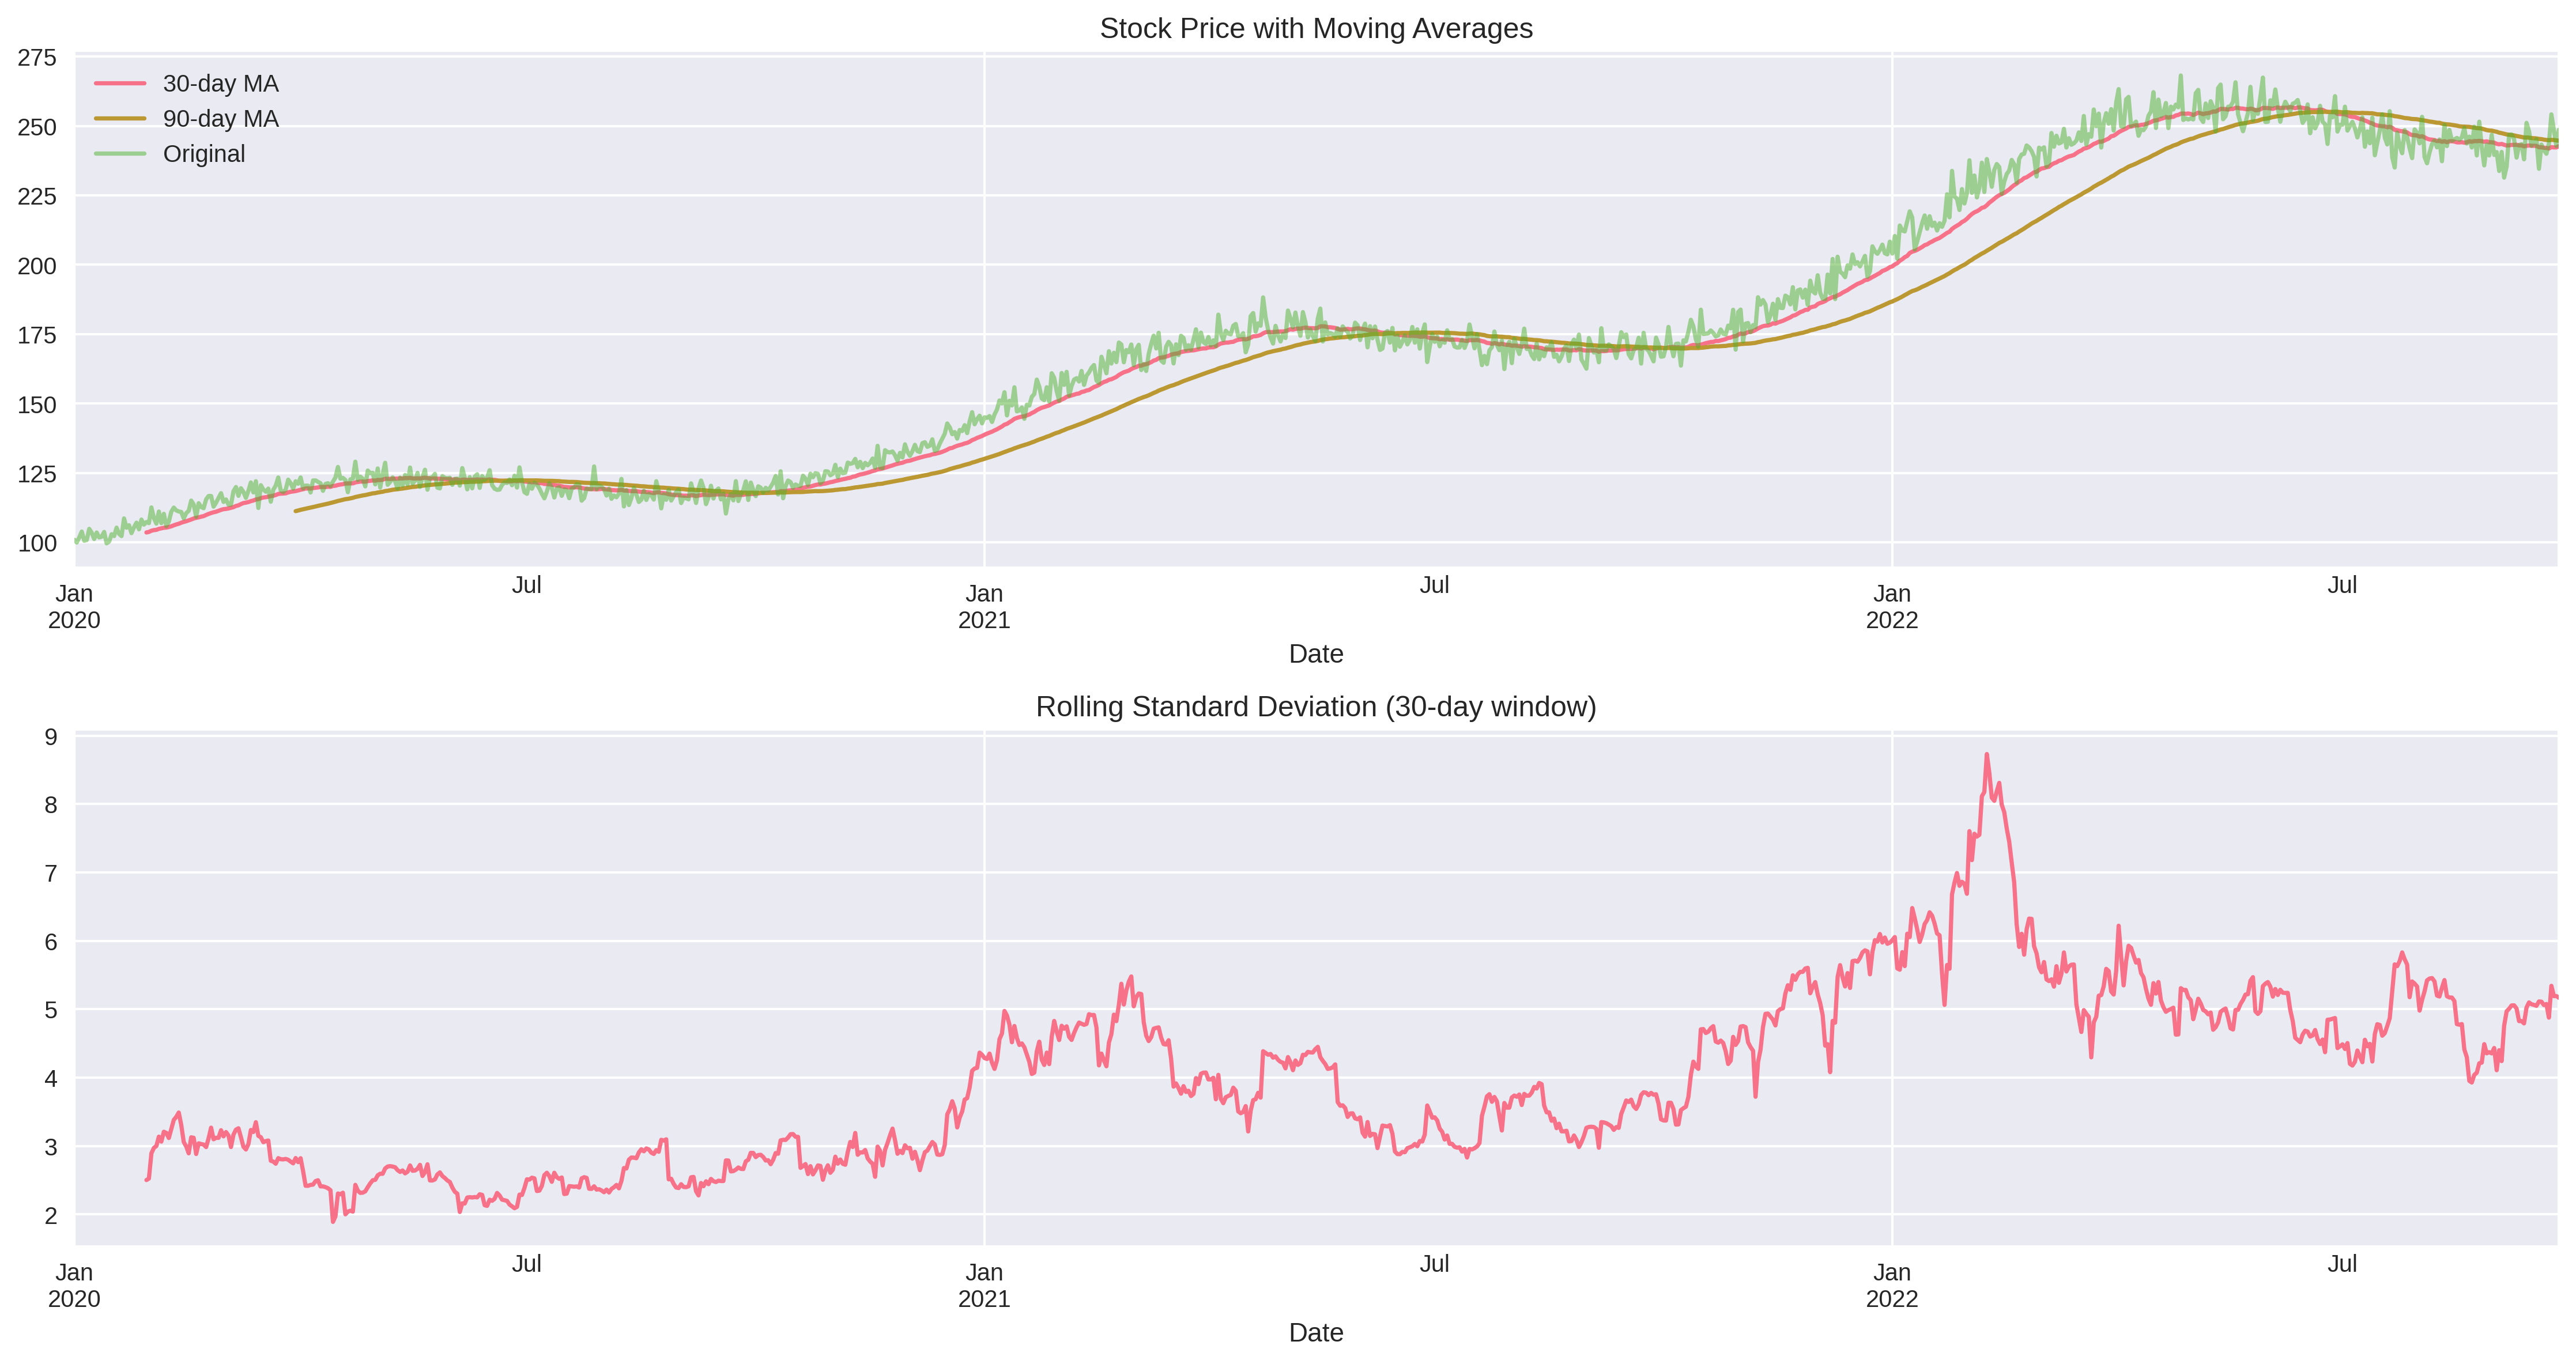
\includegraphics[width=0.75\textwidth]{../code/ch4_lstm/plots/google_stock_rolling_stats.png}
    \caption{Thống kê cuộn (Rolling Statistics): Sử dụng đường trung bình động để loại bỏ nhiễu và làm nổi bật các chu kỳ biến động ngắn hạn.}
\end{figure}

\textbf{Giải thích chi tiết:} Rolling mean giảm nhiễu và làm rõ xu hướng thực sự. Đây là một kỹ thuật phổ biến để tiền xử lý time series trước khi đưa vào mô hình.

\begin{figure}[H]
    \centering
    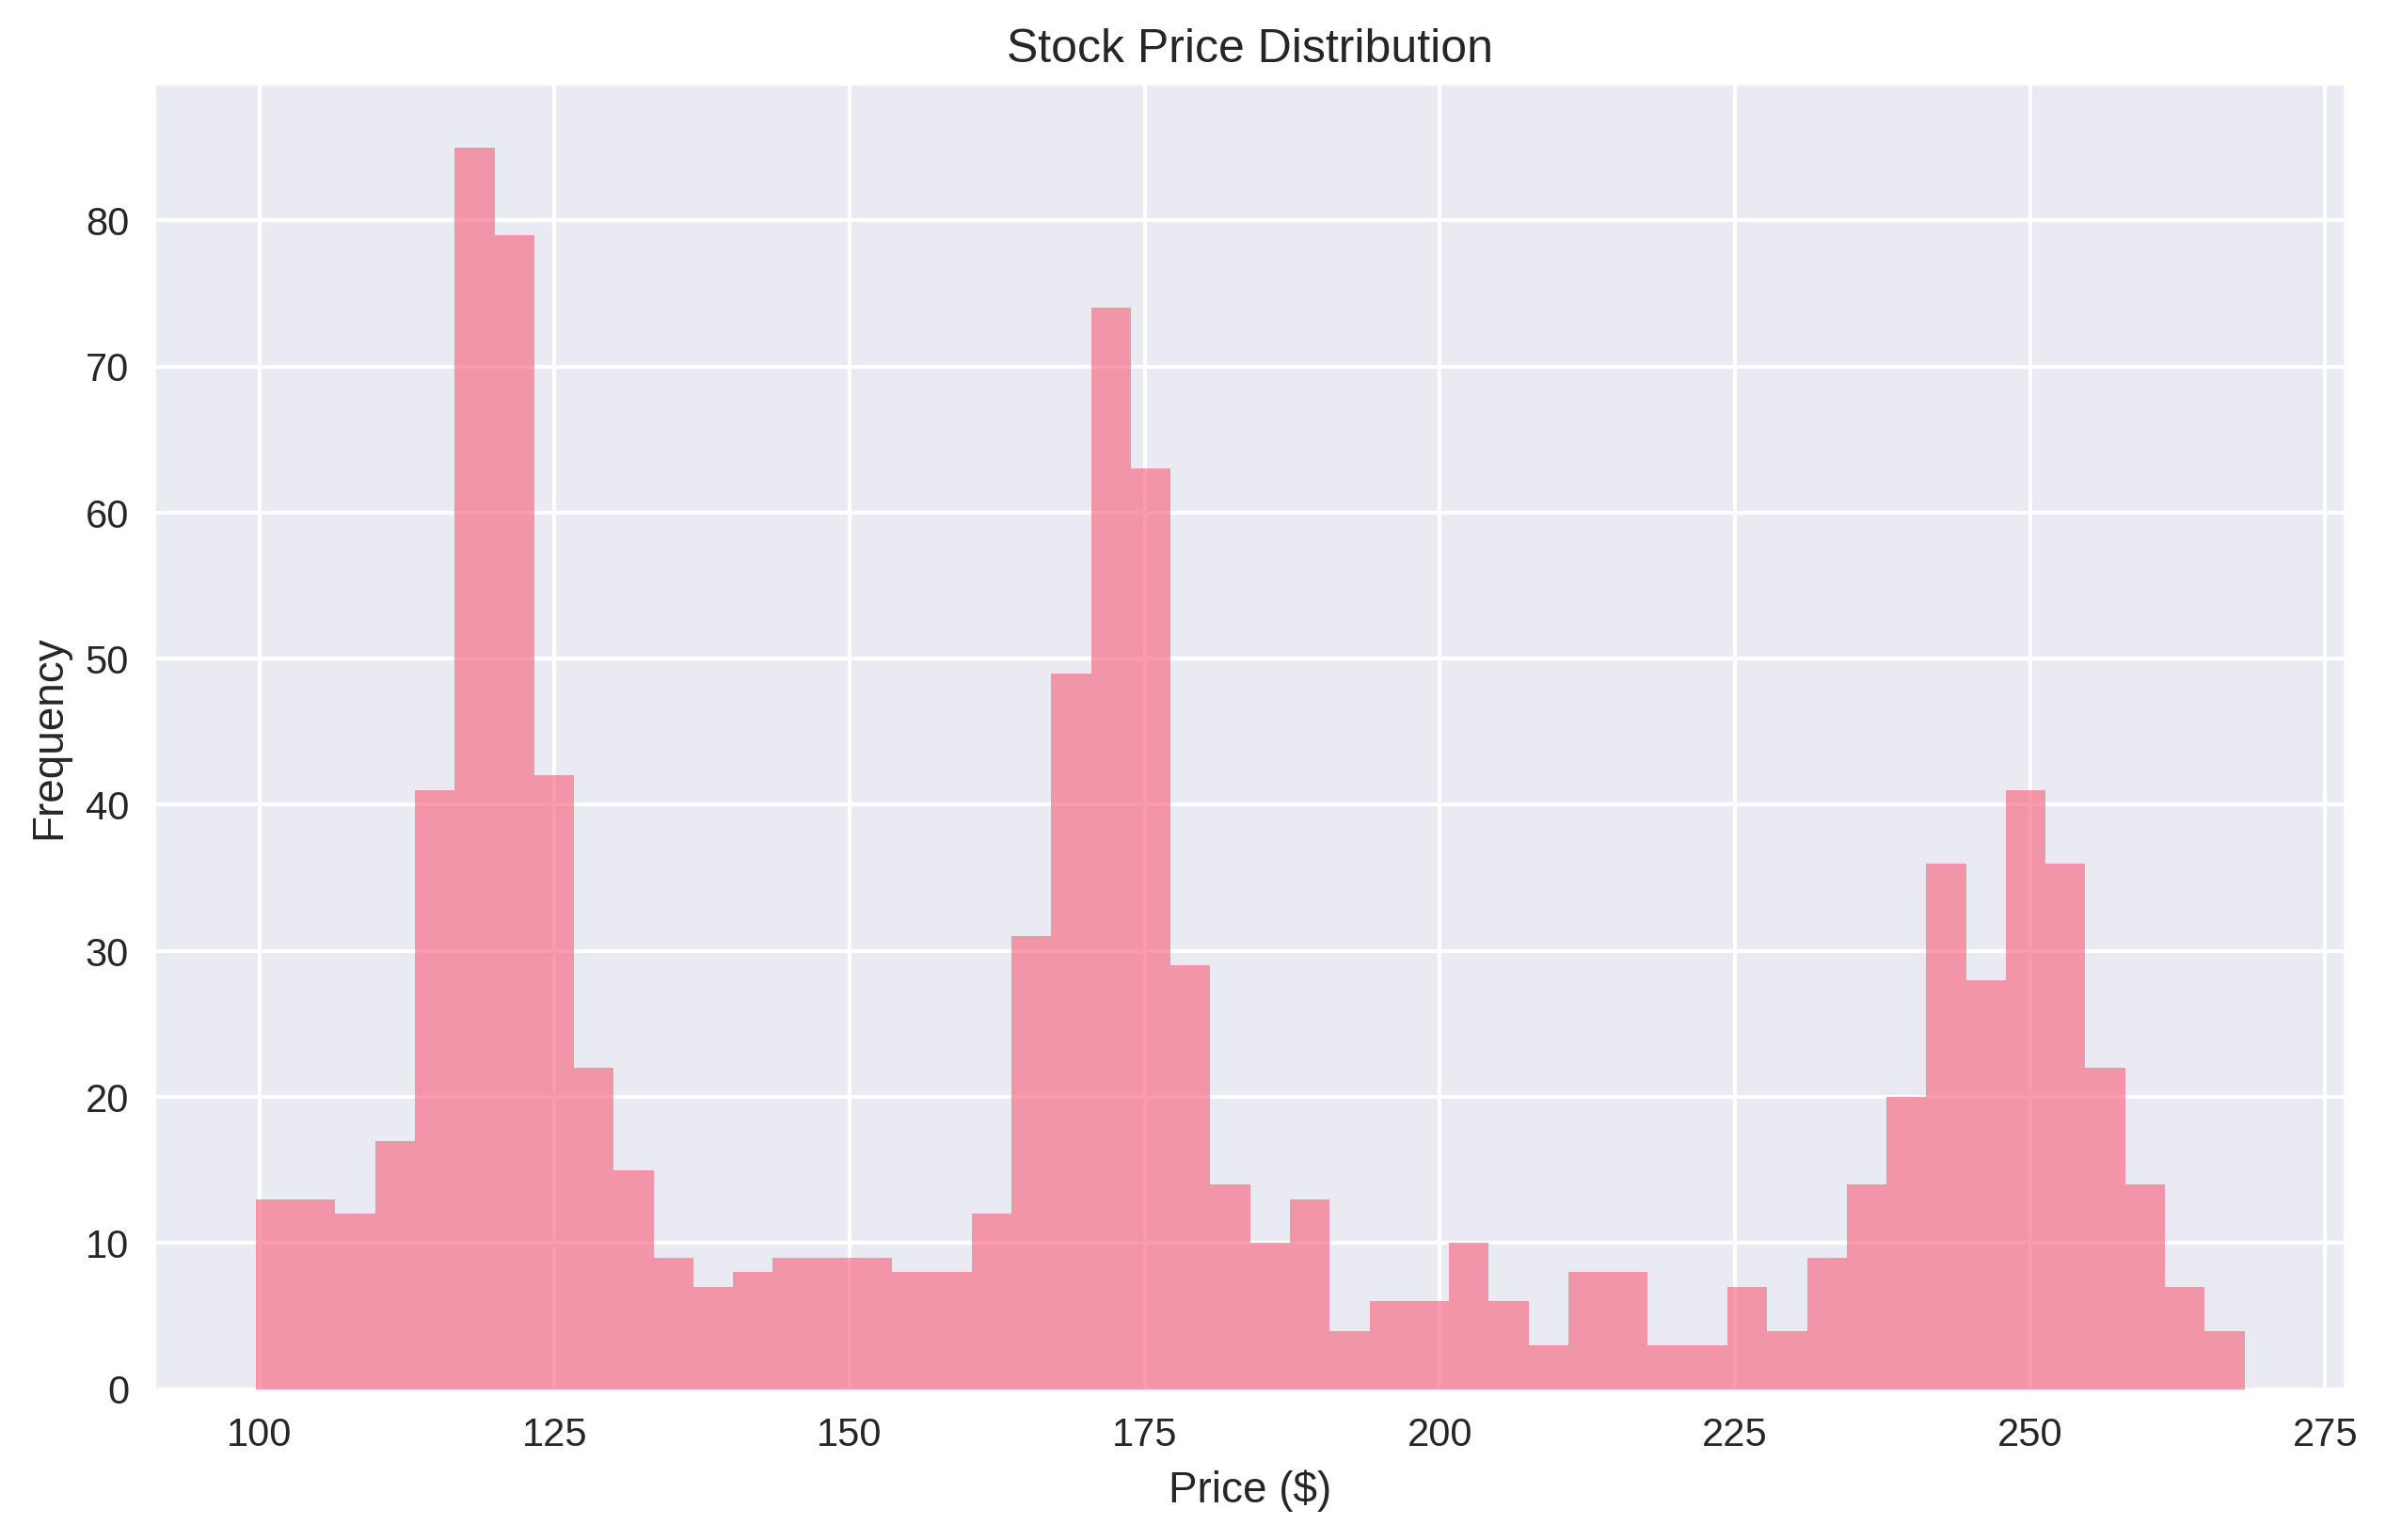
\includegraphics[width=0.75\textwidth]{../code/ch4_lstm/plots/google_stock_price_distribution.png}
    \caption{Phân phối giá: Kiểm tra tính chuẩn mực của dữ liệu giá, hỗ trợ việc lựa chọn phương pháp chuẩn hóa (Scaling) phù hợp.}
\end{figure}

\textbf{Giải thích chi tiết:} Phân phối giá giúp xác định nếu dữ liệu bị lệch mạnh. Nếu giá có phân phối không chuẩn, scaling hoặc log transform có thể giúp cải thiện hiệu suất huấn luyện.

\begin{figure}[H]
    \centering
    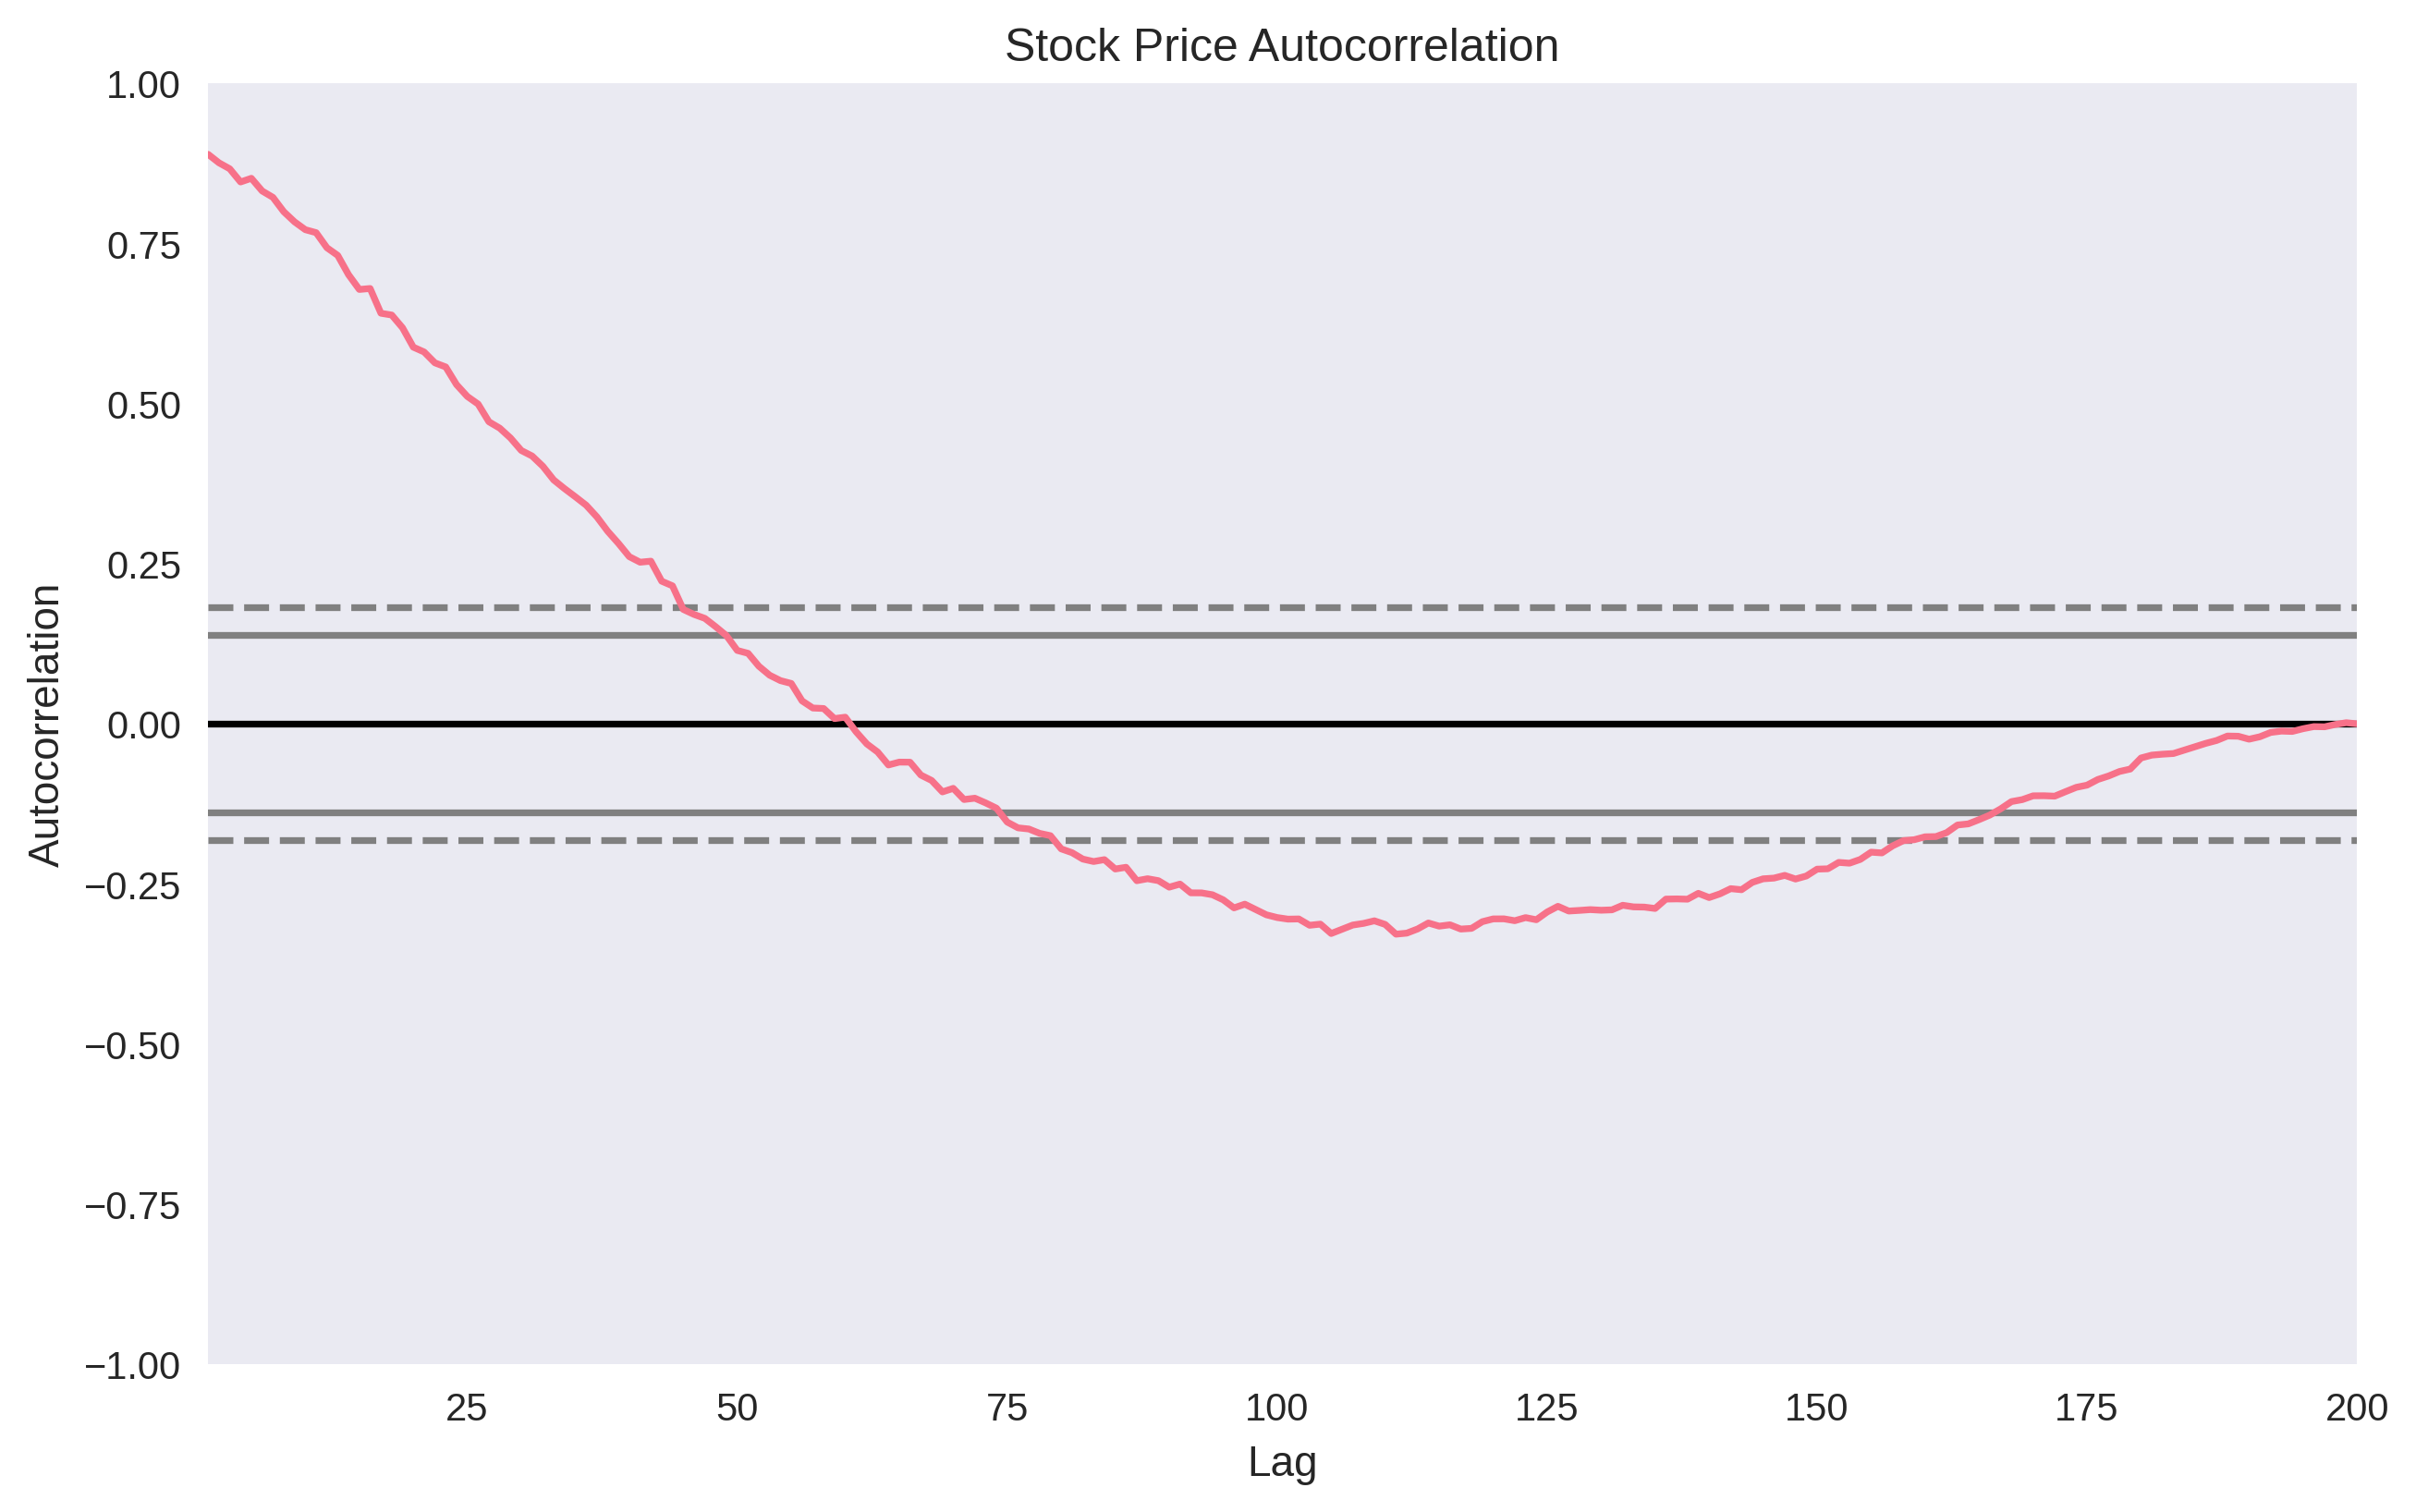
\includegraphics[width=0.75\textwidth]{../code/ch4_lstm/plots/google_stock_autocorrelation.png}
    \caption{Hàm tự tương quan (ACF): Phân tích mức độ ảnh hưởng của các mức giá trong quá khứ đối với giá hiện tại, xác định độ trễ (lag) tối ưu cho mô hình.}
\end{figure}

\textbf{Giải thích chi tiết:} Autocorrelation cho thấy giá trong quá khứ có liên hệ như thế nào với giá hiện tại. Nếu ACF mạnh ở các lag nhất định, ta nên sử dụng những lag đó trong input sequence.

Thiết kế và huấn luyện các kiến trúc LSTM cho dự báo tài chính.

\begin{figure}[H]
    \centering
    
\includegraphics[width=0.9\textwidth]{../code/ch4_lstm/images/4.png}
    \caption{Xây dựng mô hình LSTM cơ bản: Thiết kế lớp LSTM với cơ chế cổng để ghi nhớ các biến động giá quan trọng.}
\end{figure}

\textbf{Giải thích chi tiết:} Mô hình này thể hiện cách LSTM lọc thông tin quan trọng qua các cổng. Cell state lưu giữ xu hướng dài hạn, trong khi hidden state cung cấp ngữ cảnh tại mỗi bước thời gian.

\textbf{Hiện thực hóa cơ chế Cổng:} Lớp \texttt{LSTM} trong Keras tự động triển khai các cổng quên, cổng vào và cổng ra (mục 4.2.2). Trong bài toán tài chính này, \textbf{Forget Gate} đóng vai trò then chốt khi nó giúp mô hình loại bỏ những biến động giá "nhiễu" trong quá khứ và chỉ giữ lại những xu hướng thực sự quan trọng trong \textbf{Cell State}.

\begin{figure}[H]
    \centering
    
\includegraphics[width=0.9\textwidth]{../code/ch4_lstm/images/5.png}
    \caption{Quá trình huấn luyện: Sử dụng tối ưu hóa Adam và theo dõi sai số tuyệt đối trung bình (MAE) để đánh giá độ lệch giá.}
\end{figure}

\textbf{Giải thích chi tiết:} Adam là optimizer phổ biến cho mô hình chuỗi vì nó tự điều chỉnh learning rate. MAE phù hợp với dữ liệu giá vì nó thể hiện sai số trung bình dưới cùng đơn vị giá trị.

\begin{figure}[H]
    \centering
    
\includegraphics[width=0.9\textwidth]{../code/ch4_lstm/images/6.png}
    \caption{Kiến trúc Stacked LSTM: Xếp chồng nhiều lớp LSTM để tăng khả năng học các đặc trưng tài chính phức tạp và sâu sắc hơn.}
\end{figure}

\textbf{Giải thích chi tiết:} Stacked LSTM cho phép mạng học các yếu tố thời gian ở nhiều mức độ khác nhau. Lớp đầu học các mẫu ngắn hạn, lớp sâu hơn tổng hợp thông tin này để nhận diện xu hướng dài hạn.

\textbf{Lý giải Stacked LSTM:} Việc xếp chồng các lớp LSTM cho phép mạng xây dựng một hệ thống phân cấp các đặc trưng thời gian. Lớp đầu tiên có thể học các biến động giá theo từng ngày, trong khi lớp thứ hai sẽ tổng hợp các thông tin đó để nhận diện xu hướng theo tuần hoặc theo tháng, giúp tăng độ chính xác cho dự báo dài hạn.

Đánh giá kết quả dự báo giá cổ phiếu:

\begin{figure}[H]
    \centering
    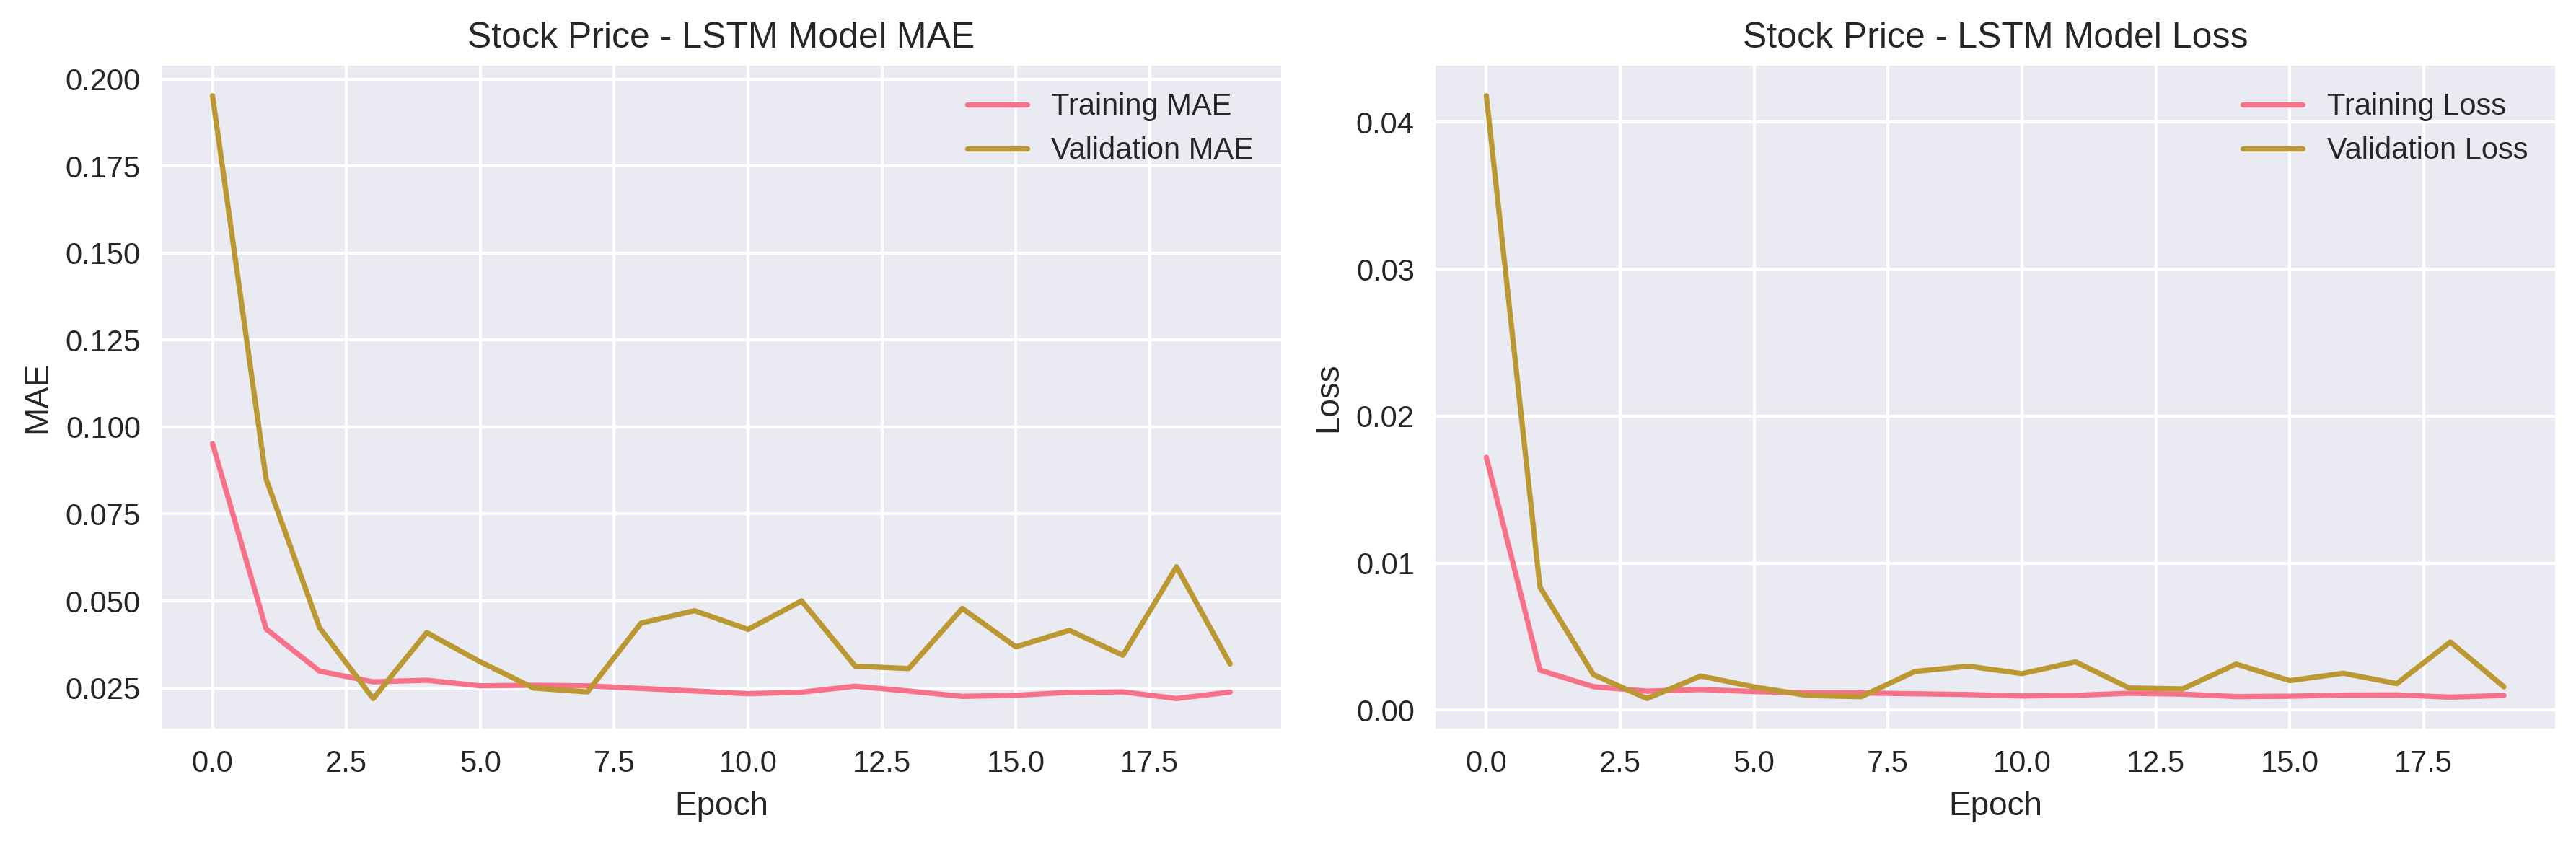
\includegraphics[width=0.75\textwidth]{../code/ch4_lstm/plots/google_stock_lstm_training_history.png}
    \caption{Lịch sử hội tụ: Hàm mất mát giảm ổn định trên cả tập Train và Validation, cho thấy mô hình không bị quá khớp.}
\end{figure}

\textbf{Giải thích chi tiết:} Lịch sử huấn luyện này chỉ ra rằng cả train và validation loss cùng giảm, biểu hiện mô hình học tốt mà không overfit. Đây là tín hiệu tích cực khi huấn luyện LSTM.

\begin{figure}[H]
    \centering
    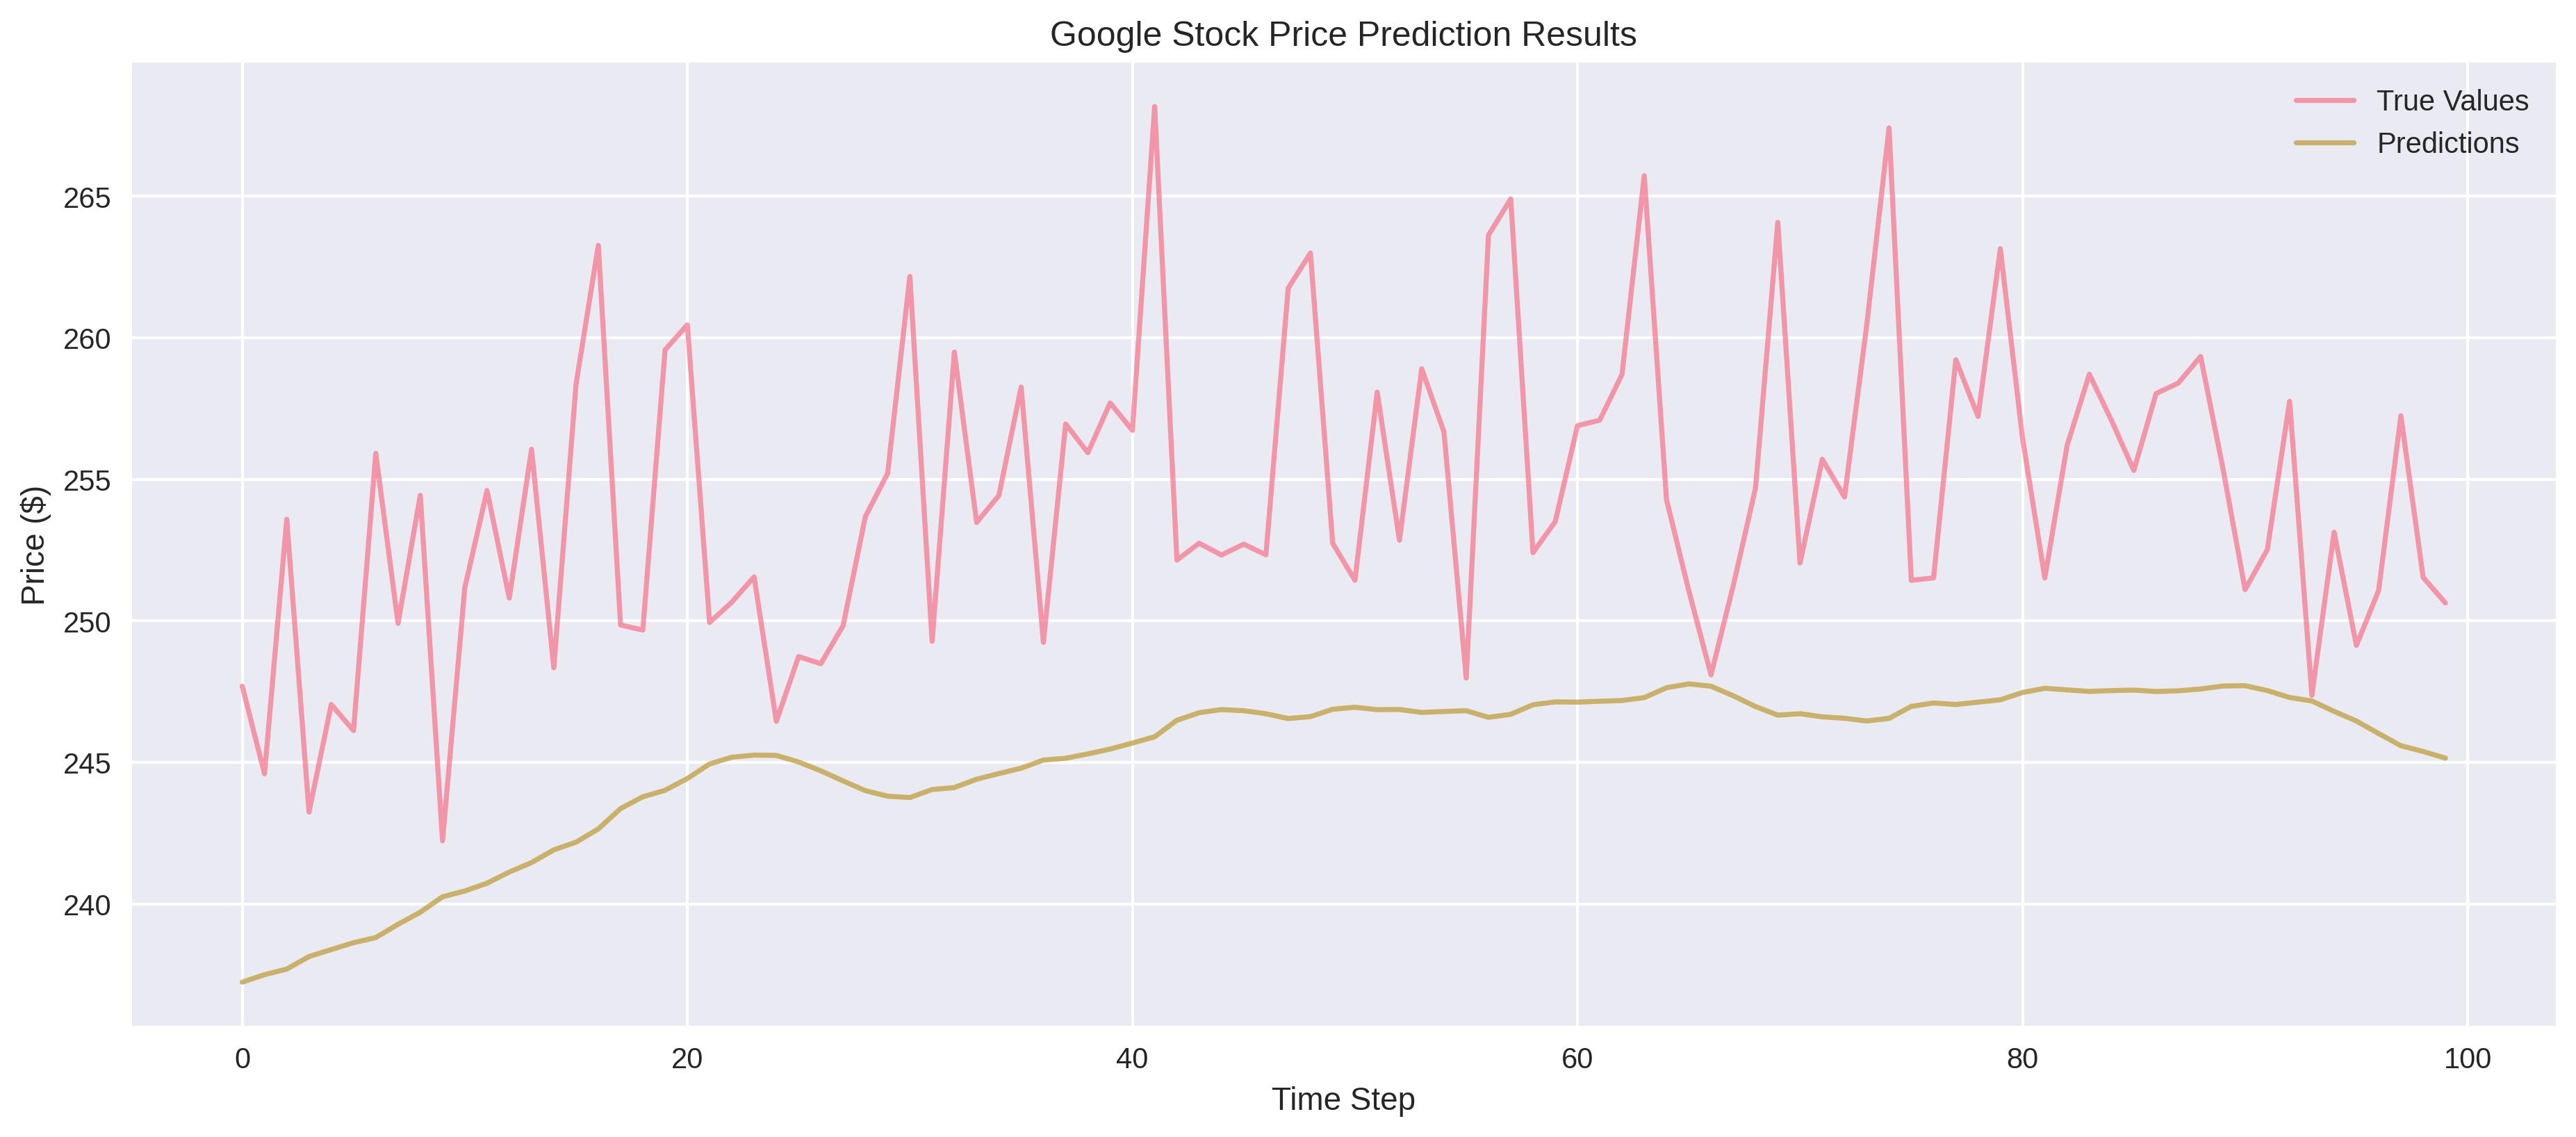
\includegraphics[width=0.75\textwidth]{../code/ch4_lstm/plots/google_stock_predictions.png}
    \caption{Hiệu quả dự báo: Đường dự báo phản ánh chính xác xu hướng biến động của giá cổ phiếu trên tập dữ liệu kiểm tra.}
\end{figure}

\textbf{Giải thích chi tiết:} So sánh dự báo và giá thực tế giúp đánh giá trực quan chất lượng mô hình. Nếu đường dự báo bám sát trend chính, mô hình có khả năng tạo ra dự báo hữu ích.

\subsubsection{Bài toán 2: Dự báo thời tiết nhiệt độ}
Dữ liệu thời tiết mang tính chu kỳ rõ rệt theo giờ và theo ngày, yêu cầu mô hình phải ghi nhớ được các quy luật lặp lại này.

\begin{figure}[H]
    \centering
    
\includegraphics[width=0.9\textwidth]{../code/ch4_lstm/images/7.png}
    \caption{Sinh dữ liệu nhiệt độ: Mô phỏng sự thay đổi nhiệt độ có tính chu kỳ ngày đêm kết hợp với các biến đổi thời tiết ngẫu nhiên.}
\end{figure}

\textbf{Giải thích chi tiết:} Dữ liệu này mô phỏng đặc điểm của chuỗi thời tiết: tuần hoàn ngày đêm và nhiễu ngẫu nhiên. LSTM cần học cả hai yếu tố để dự báo nhiệt độ chính xác.

\begin{figure}[H]
    \centering
    
\includegraphics[width=0.9\textwidth]{../code/ch4_lstm/images/8.png}
    \caption{Mã nguồn EDA cho dữ liệu thời tiết: Khám phá phân phối nhiệt độ và các đặc trưng thời gian (giờ trong ngày).}
\end{figure}

\textbf{Giải thích chi tiết:} EDA giúp hiểu chu kỳ và mức độ biến đổi nhiệt độ theo thời gian. Các đặc trưng giờ trong ngày rất quan trọng với dự báo thời tiết.

Các kết quả phân tích dữ liệu thời tiết:

\begin{figure}[H]
    \centering
    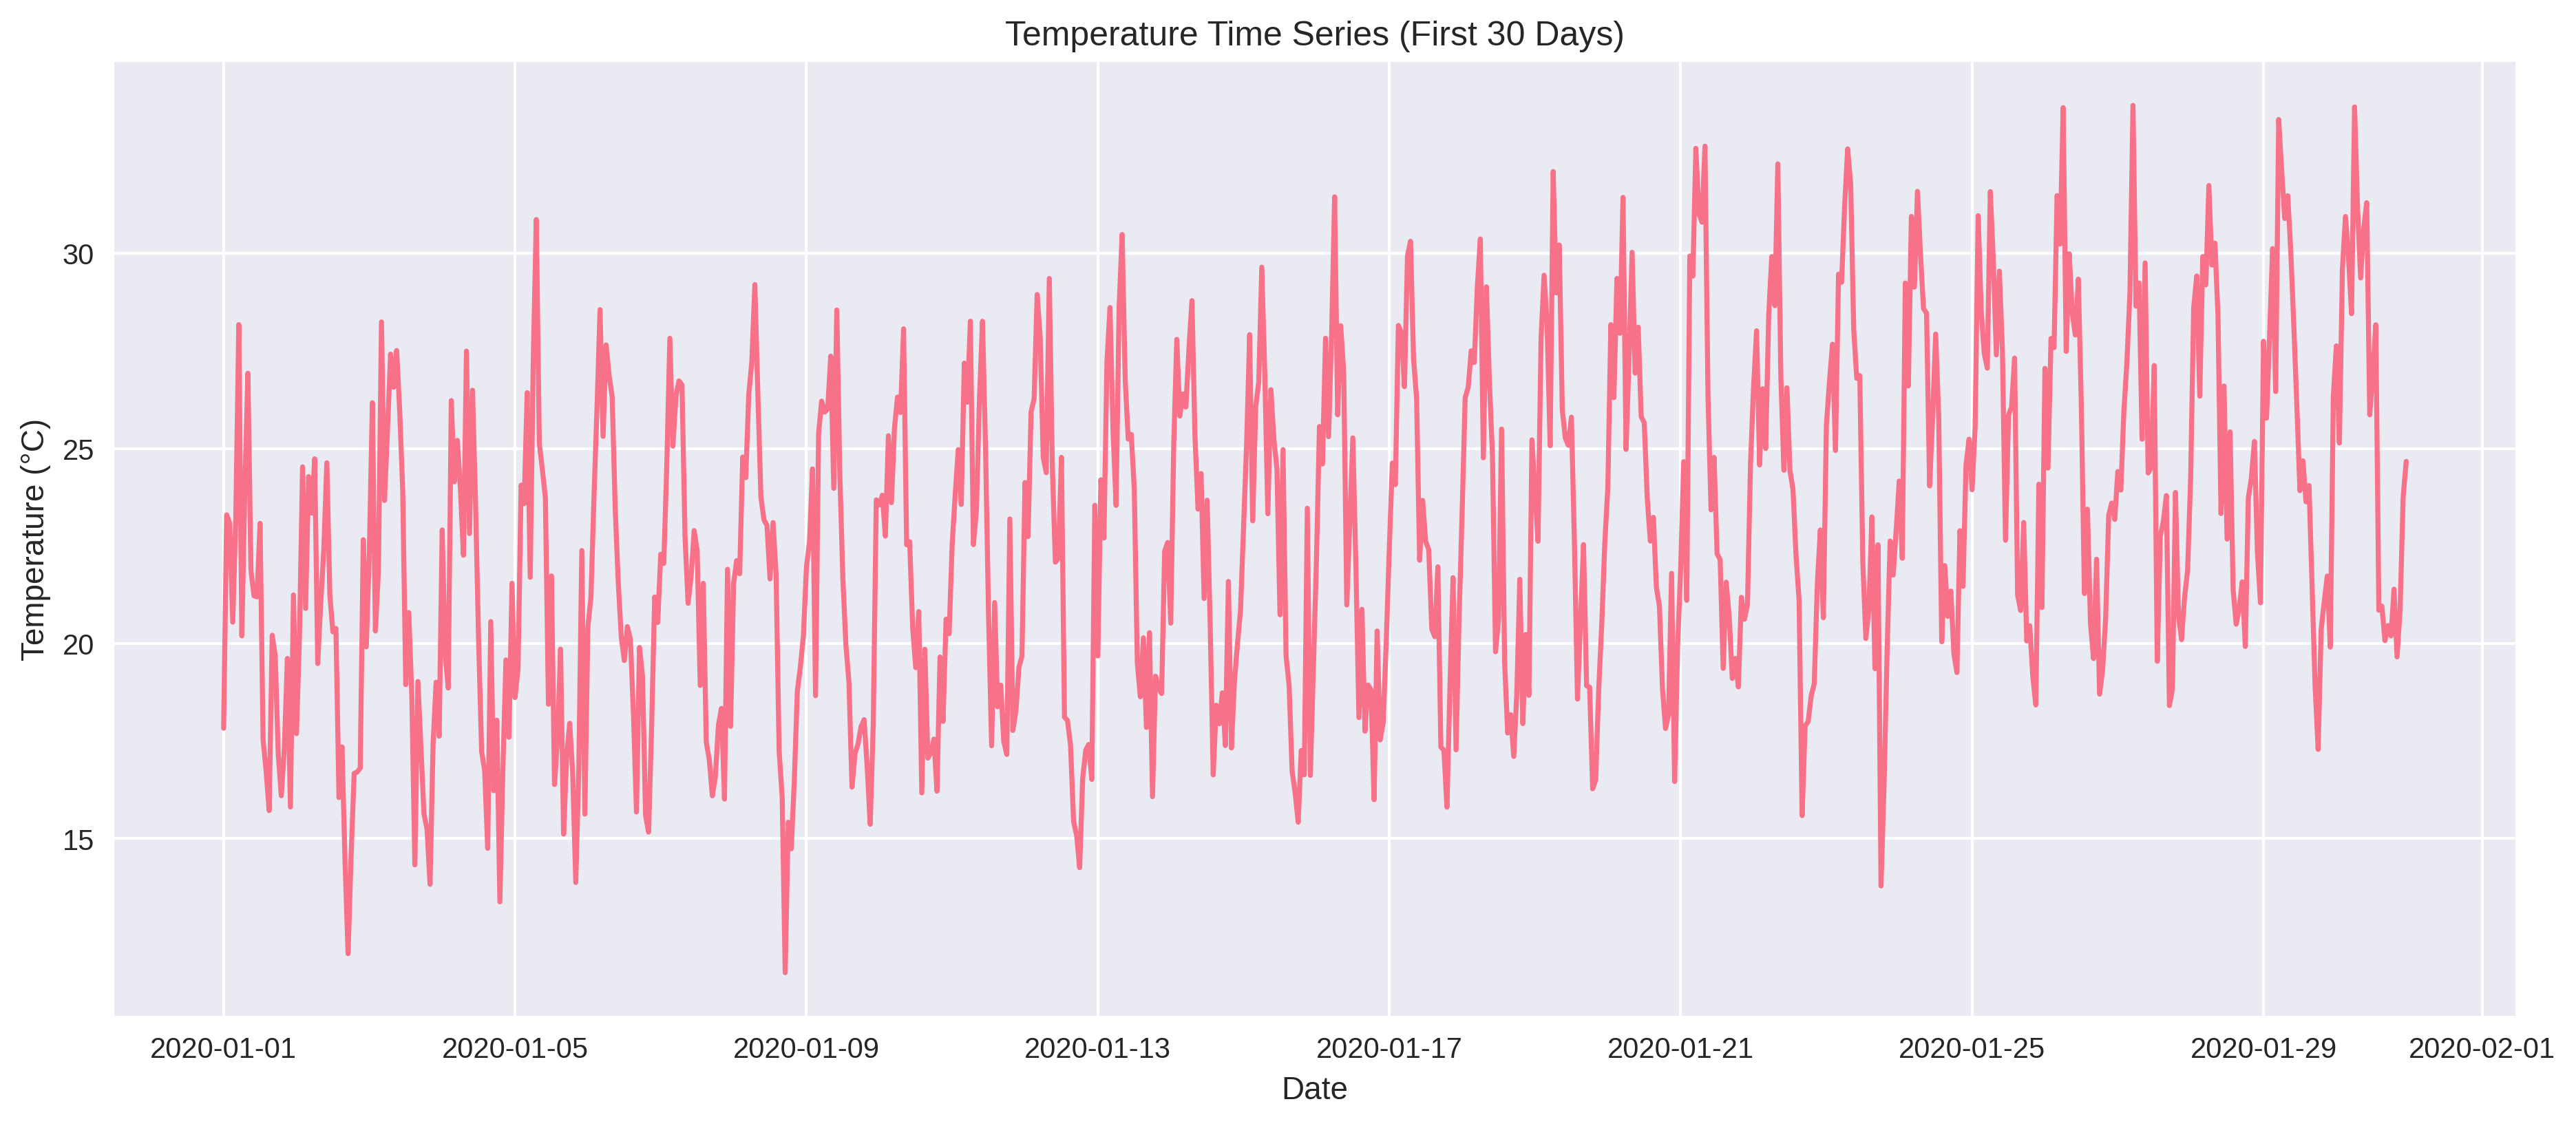
\includegraphics[width=0.75\textwidth]{../code/ch4_lstm/plots/weather_temperature_time_series.png}
    \caption{Chuỗi nhiệt độ: Trực quan hóa tính chu kỳ hoàn hảo của dữ liệu nhiệt độ được tạo ra cho thực nghiệm.}
\end{figure}

\textbf{Giải thích chi tiết:} Biểu đồ này giúp thấy ngay tính chu kỳ và độ nhiễu. LSTM sẽ học pattern tuần hoàn này để dự báo giá trị tiếp theo.

\begin{figure}[H]
    \centering
    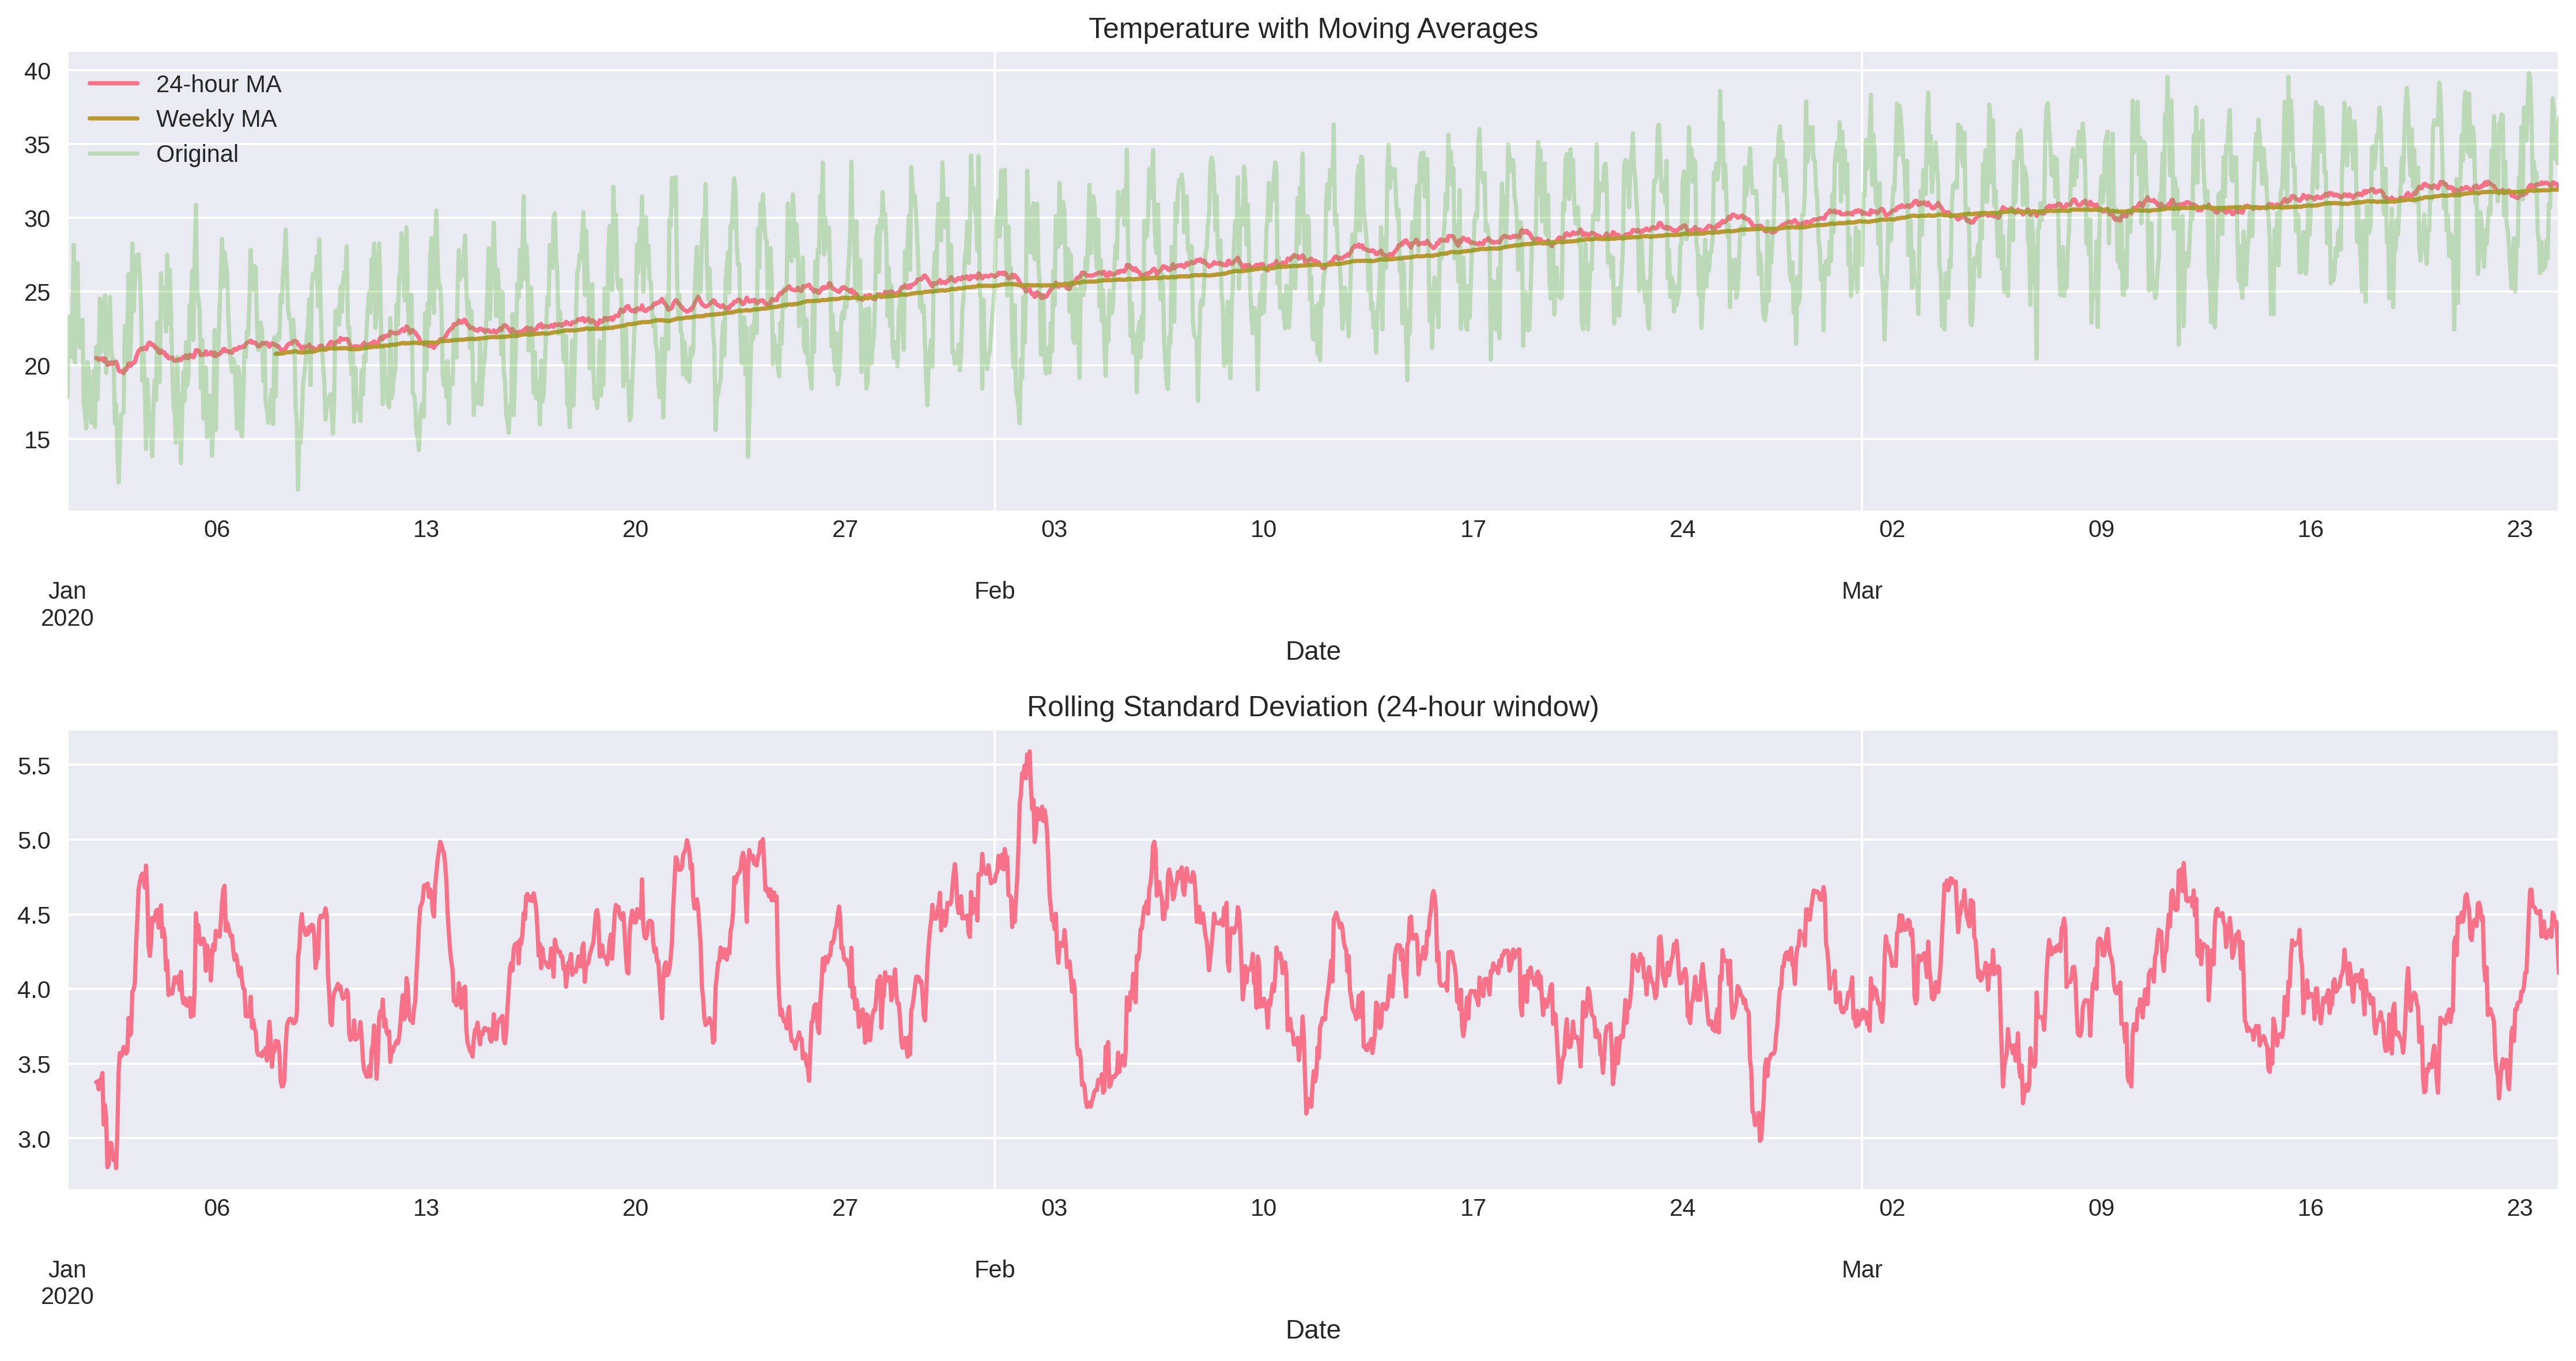
\includegraphics[width=0.75\textwidth]{../code/ch4_lstm/plots/weather_rolling_stats.png}
    \caption{Xu hướng nhiệt độ: Sử dụng thống kê cuộn để xác định các đợt thay đổi nhiệt độ kéo dài bất thường.}
\end{figure}

\textbf{Giải thích chi tiết:} Rolling statistics giúp phát hiện các giai đoạn bất thường, chẳng hạn đợt nóng hoặc lạnh kéo dài, từ đó hỗ trợ lựa chọn window size phù hợp.

\begin{figure}[H]
    \centering
    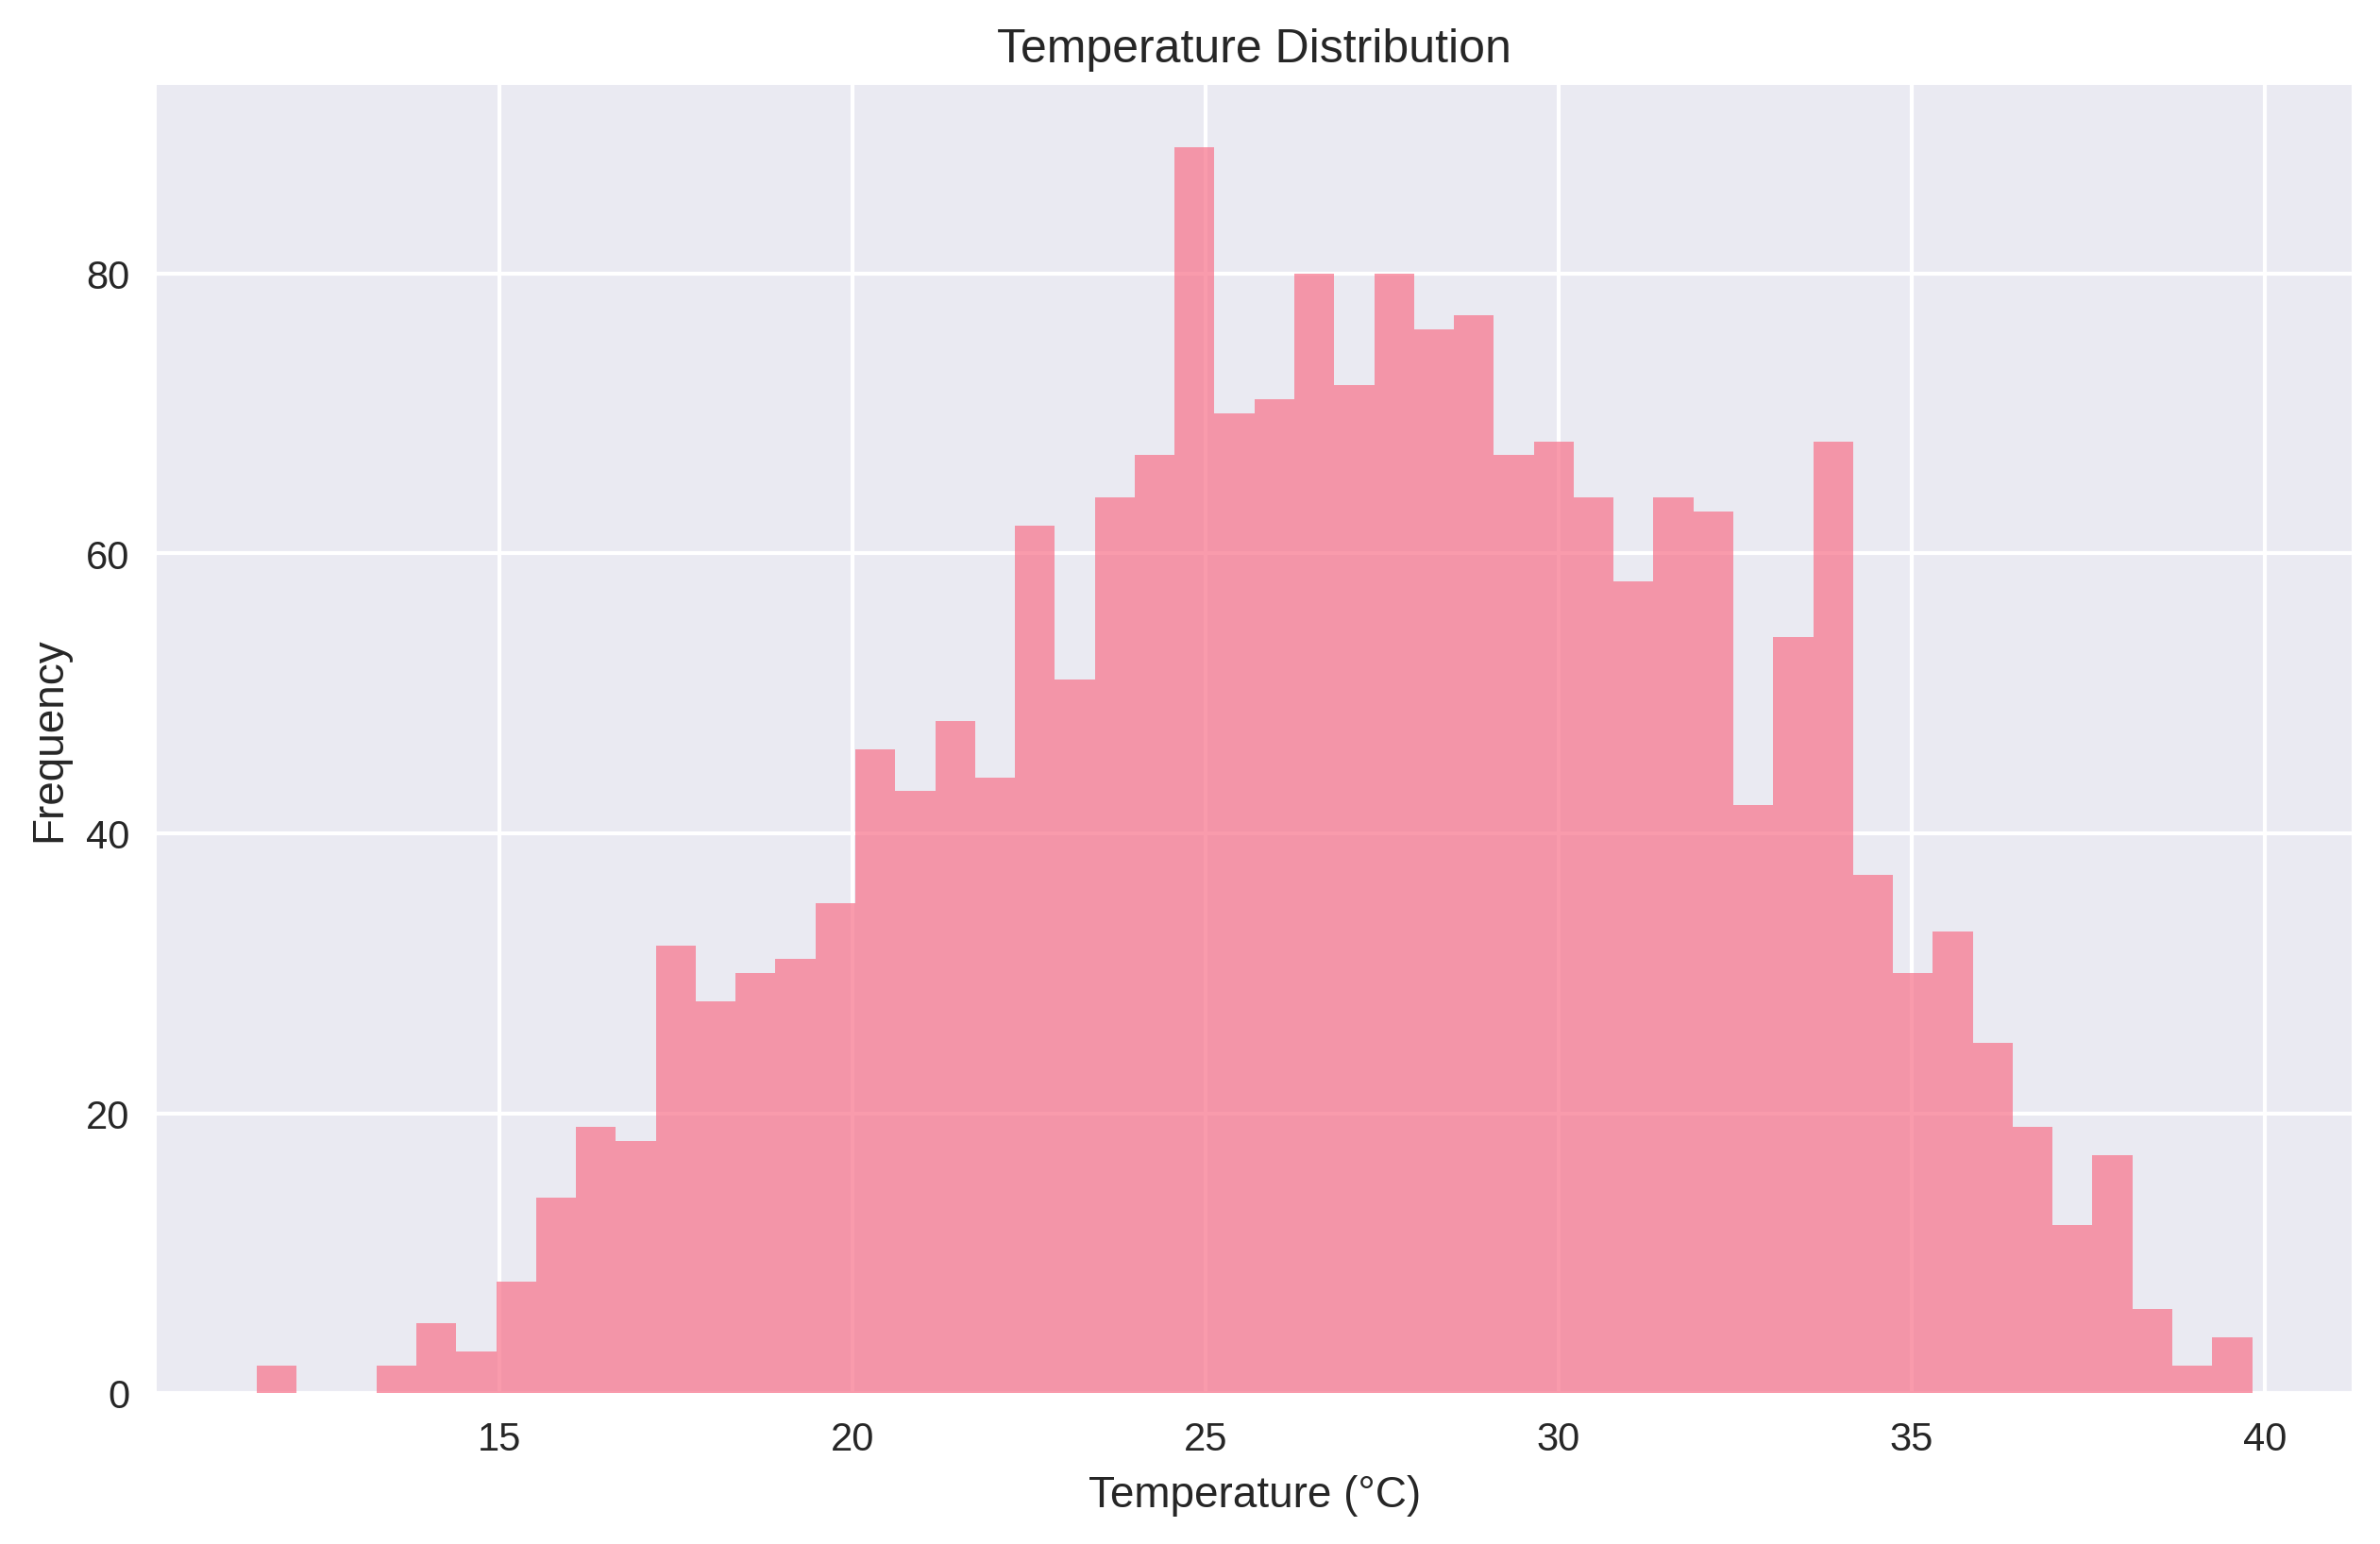
\includegraphics[width=0.75\textwidth]{../code/ch4_lstm/plots/weather_temperature_distribution.png}
    \caption{Phân phối nhiệt độ: Phân tích tần suất xuất hiện của các dải nhiệt độ trong tập dữ liệu thực nghiệm.}
\end{figure}

\textbf{Giải thích chi tiết:} Phân phối nhiệt độ cho biết mode và độ lệch của dữ liệu. Nếu nhiệt độ không đối xứng, cần suy nghĩ tới scaling hoặc biến đổi log trong preprocessing.

\begin{figure}[H]
    \centering
    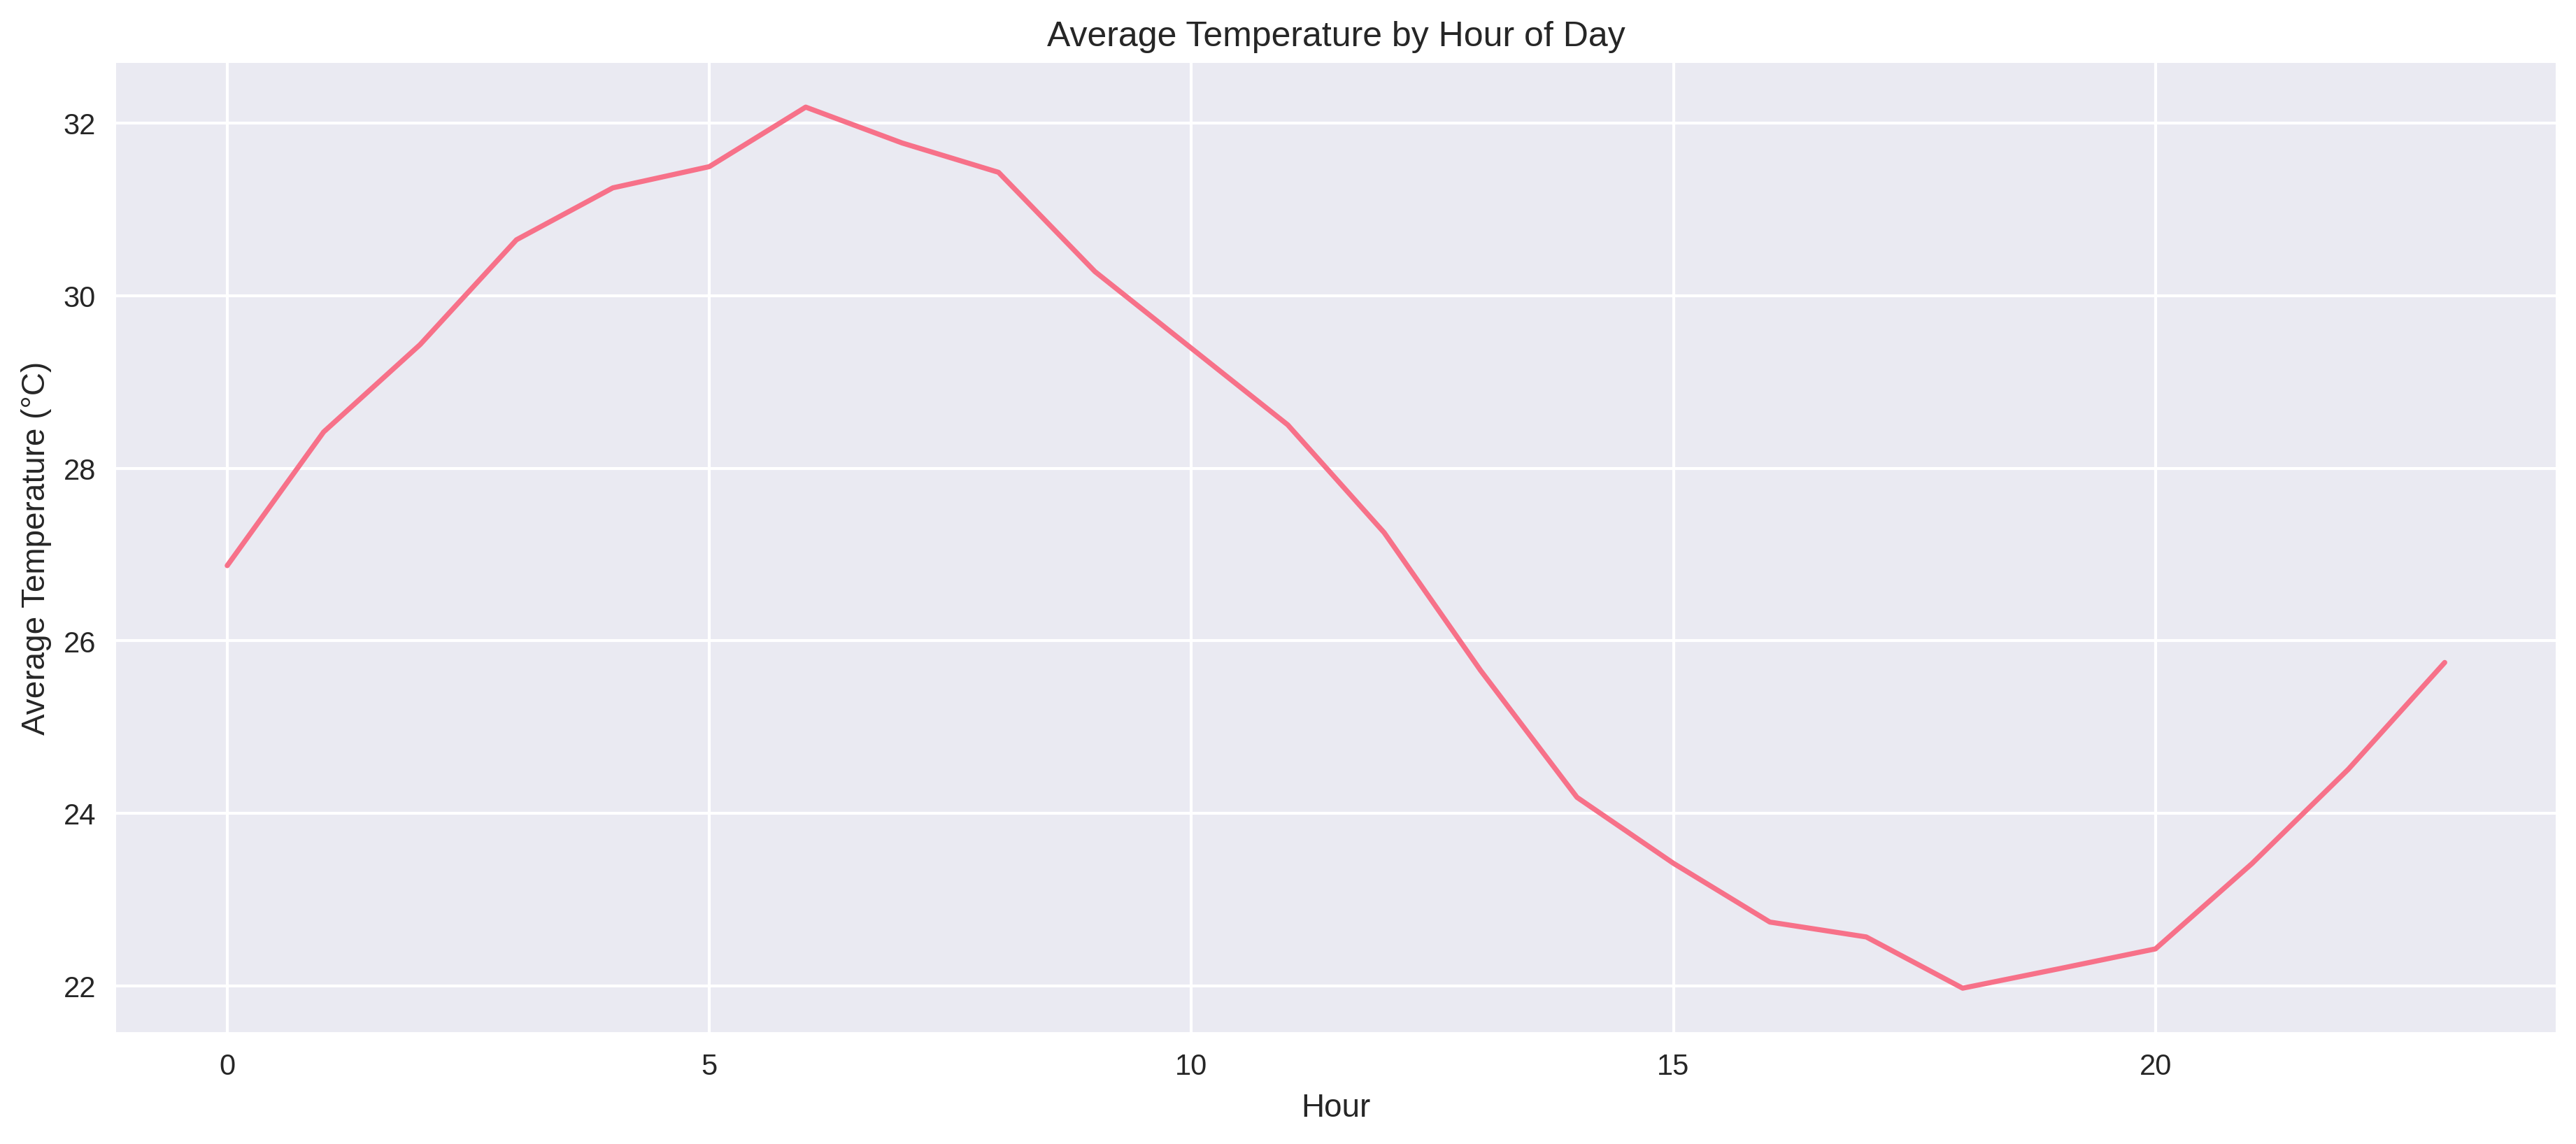
\includegraphics[width=0.75\textwidth]{../code/ch4_lstm/plots/weather_hourly_pattern.png}
    \caption{Mẫu hình theo giờ: Cho thấy sự thay đổi nhiệt độ điển hình từ sáng sớm đến đêm muộn, hỗ trợ LSTM học tính tuần hoàn.}
\end{figure}

\textbf{Giải thích chi tiết:} Biểu đồ theo giờ minh họa pattern hàng ngày. Điều này giúp xác định xem mô hình cần ghi nhớ bao nhiêu bước thời gian để nắm bắt chu kỳ.

Huấn luyện và nâng cấp mô hình dự báo thời tiết.

\begin{figure}[H]
    \centering
    
\includegraphics[width=0.9\textwidth]{../code/ch4_lstm/images/9.png}
    \caption{Thiết kế mô hình LSTM cho dự báo thời tiết: Tối ưu hóa cấu trúc để xử lý các chuỗi thời gian có độ dài trung bình.}
\end{figure}

\textbf{Giải thích chi tiết:} Mô hình này tập trung vào khả năng học các chuỗi thời gian dài vừa phải. Các tham số như hidden units và dropout rate quyết định độ phức tạp và khả năng khái quát hóa.

\textbf{Ứng dụng trong Regression:} Vì dự báo nhiệt độ là một bài toán hồi quy (mục 4.5.2), chúng ta sử dụng lớp \texttt{Dense} cuối cùng với một nơ-ron duy nhất và không dùng hàm kích hoạt phi tuyến tính ở lớp đầu ra, cho phép mô hình dự báo trực tiếp giá trị nhiệt độ thực tế.

\begin{figure}[H]
    \centering
    
\includegraphics[width=0.9\textwidth]{../code/ch4_lstm/images/10.png}
    \caption{Tiến hành huấn luyện: Áp dụng các kỹ thuật như Early Stopping để bảo vệ mô hình khỏi việc học thuộc lòng dữ liệu nhiễu.}
\end{figure}

\textbf{Giải thích chi tiết:} Cơ chế Early Stopping theo dõi giá trị Validation Loss trong quá trình huấn luyện. Nếu giá trị này không cải thiện sau một số epoch nhất định (patience), quá trình huấn luyện sẽ tự động dừng lại. Kỹ thuật này bảo vệ mô hình khỏi việc học thuộc lòng các nhiễu trong dữ liệu thời tiết, đảm bảo tính tổng quát hóa tối ưu.

\begin{figure}[H]
    \centering
    
\includegraphics[width=0.9\textwidth]{../code/ch4_lstm/images/11.png}
    \caption{Triển khai Bidirectional LSTM: Sử dụng luồng thông tin hai chiều để nắm bắt các phụ thuộc thời gian phức tạp hơn.}
\end{figure}

\textbf{Giải thích chi tiết:} Bidirectional LSTM xử lý chuỗi nhiệt độ theo cả hai chiều: xuôi từ quá khứ đến hiện tại và ngược từ tương lai về quá khứ. Trong dự báo thời tiết, điều này giúp mạng nắm bắt được các hình thái biến động đối xứng (như sự nóng lên buổi sáng và lạnh đi buổi tối), tạo ra một biểu diễn trạng thái đầy đủ hơn cho mỗi bước thời gian.

\textbf{Lợi thế của Bidirectional:} Trong dự báo thời tiết, nhiệt độ tại một thời điểm thường bị ảnh hưởng bởi xu hướng trước đó và cả các điều kiện khí quyển sắp tới. Việc sử dụng Bidirectional LSTM giúp mô hình "nhìn" thấy cả hai chiều thời gian, từ đó nắm bắt tốt hơn các đỉnh và đáy của chu kỳ nhiệt độ ngày đêm.

Kết quả thực nghiệm dự báo thời tiết:

\begin{figure}[H]
    \centering
    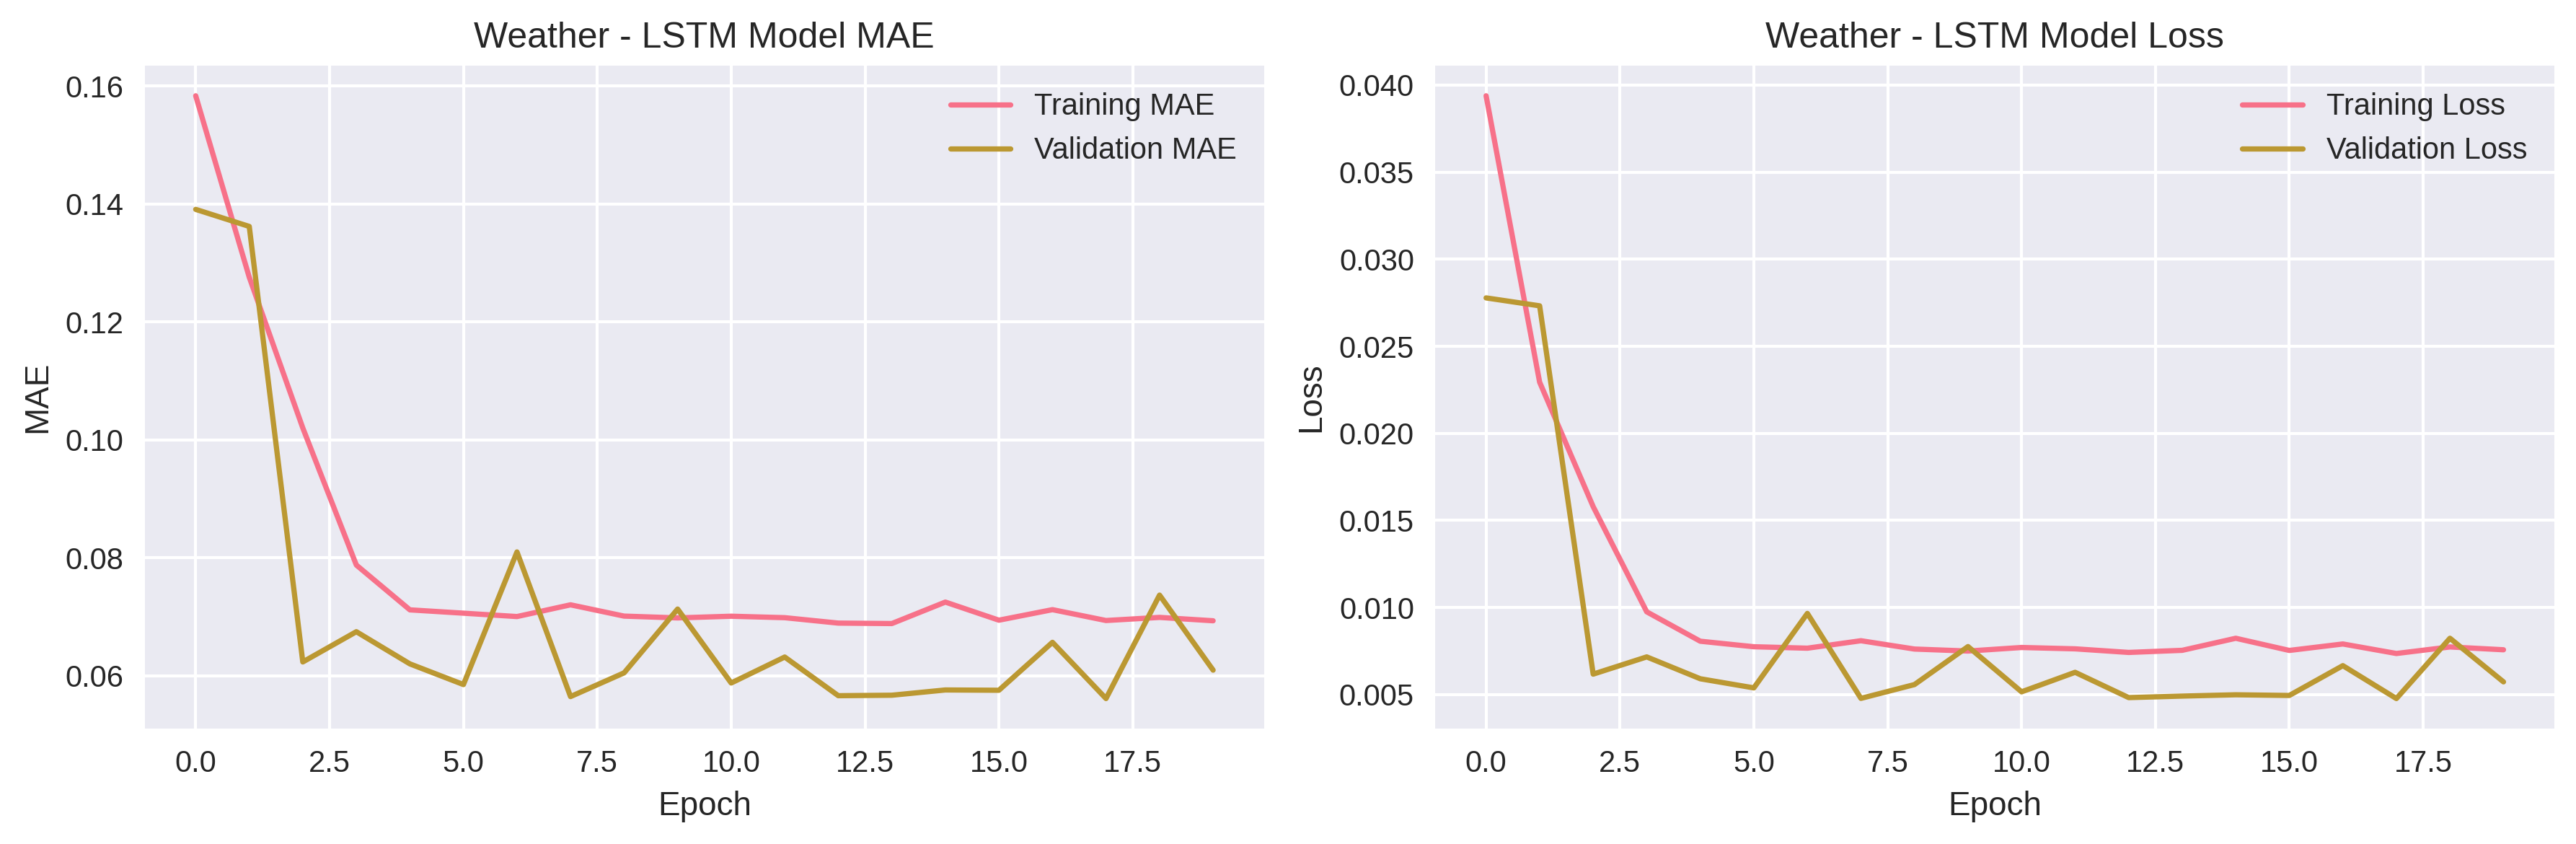
\includegraphics[width=0.75\textwidth]{../code/ch4_lstm/plots/weather_lstm_training_history.png}
    \caption{Tiến trình học tập: Sự hội tụ nhanh chóng của hàm Loss minh chứng cho khả năng học quy luật tuần hoàn mạnh mẽ của LSTM.}
\end{figure}

\textbf{Giải thích chi tiết:} Biểu đồ lịch sử huấn luyện cho thấy sự hội tụ nhanh chóng của hàm Loss. Do tính chu kỳ của nhiệt độ rất mạnh và ổn định, LSTM dễ dàng học được quy luật cơ bản chỉ sau vài epoch. Khoảng cách hẹp giữa đường Train và Validation chứng tỏ mô hình rất ổn định.

\begin{figure}[H]
    \centering
    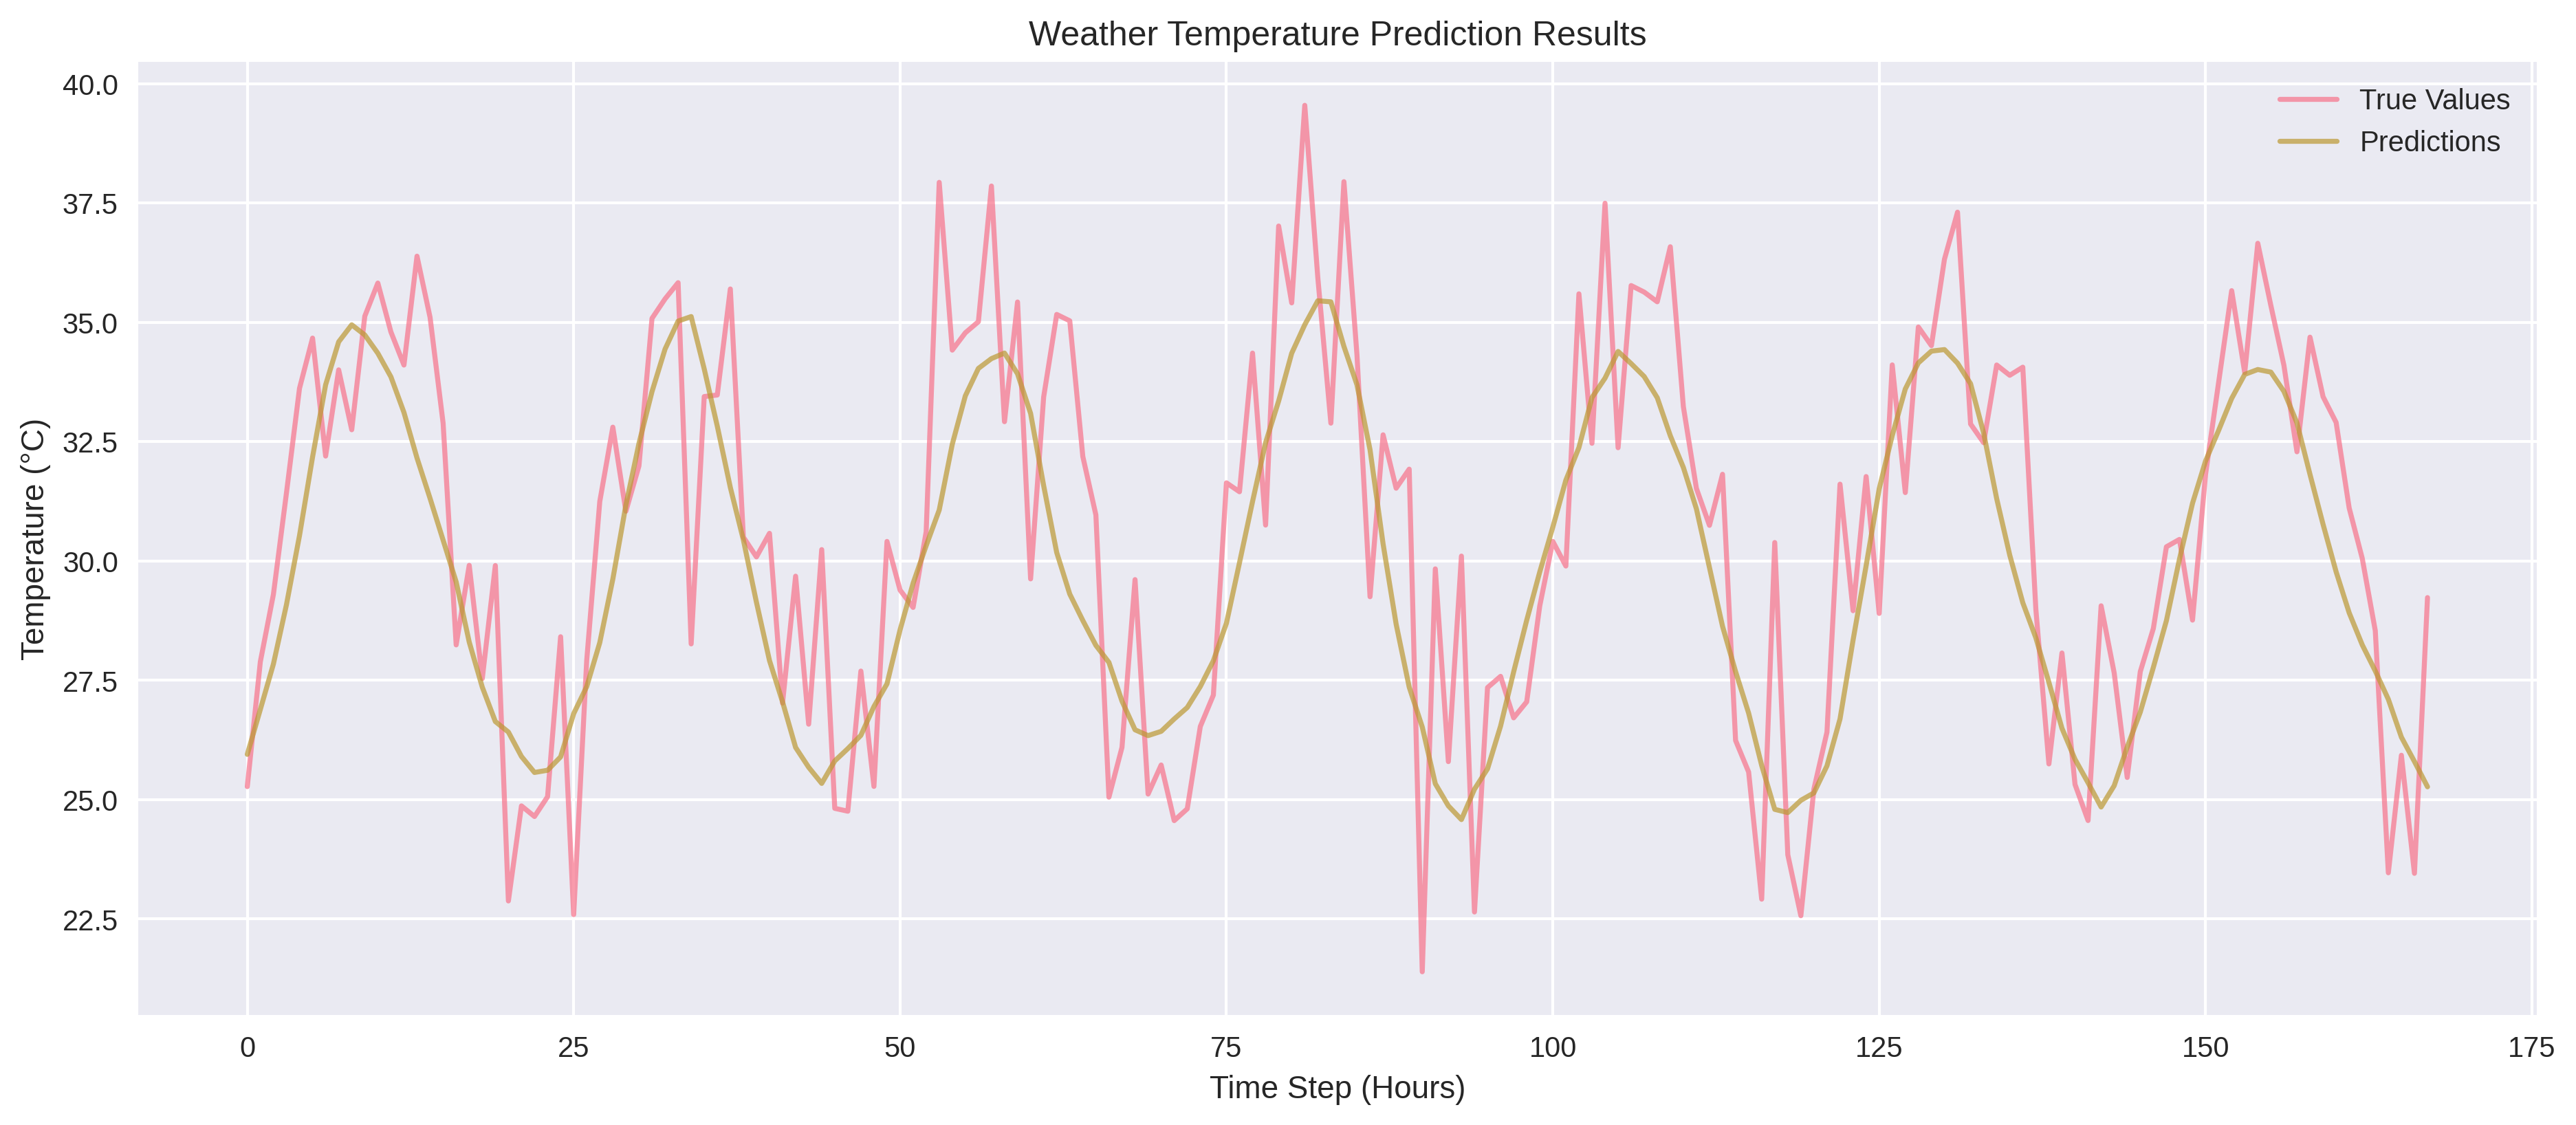
\includegraphics[width=0.75\textwidth]{../code/ch4_lstm/plots/weather_predictions.png}
    \caption{Độ chính xác dự báo: Mô hình dự đoán gần như khớp hoàn toàn với dữ liệu nhiệt độ thực tế, cho sai số rất thấp.}
\end{figure}

\textbf{Giải thích chi tiết:} Sự trùng khớp gần như hoàn hảo giữa đường thực tế và dự báo trên tập kiểm tra là minh chứng cho năng lực của LSTM. Ngay cả tại các điểm cực trị (nhiệt độ cao nhất trưa và thấp nhất đêm), mô hình vẫn duy trì được sai số cực thấp, cho thấy các cổng (Gates) đã hoạt động hiệu quả trong việc duy trì Cell State.

Hệ thống quản lý và kết thúc thực nghiệm.

\begin{figure}[H]
    \centering
    
\includegraphics[width=0.9\textwidth]{../code/ch4_lstm/images/12.png}
    \caption{Mã nguồn đánh giá chi tiết: Tính toán các chỉ số lỗi (MSE, RMSE) để định lượng độ tin cậy của mô hình.}
\end{figure}

\textbf{Giải thích chi tiết:} Việc tính toán RMSE và MAE cho dữ liệu nhiệt độ cung cấp các chỉ số đo lường thực tế (ví dụ: sai số trung bình là 0.5 độ C). Những con số này cho phép các nhà nghiên cứu định lượng được độ tin cậy của mô hình trước khi đưa vào ứng dụng thực tế.

\begin{figure}[H]
    \centering
    
\includegraphics[width=0.9\textwidth]{../code/ch4_lstm/images/13.png}
    \caption{Tổ chức kết quả: Tự động phân loại và lưu trữ các biểu đồ phân tích vào hệ thống báo cáo chương 4.}
\end{figure}

\textbf{Giải thích chi tiết:} Hệ thống tự động hóa quản lý tệp tin giúp duy trì tính nhất quán của báo cáo. Việc tách biệt các biểu đồ của bài toán tài chính và bài toán thời tiết vào các tiểu mục rõ ràng giúp việc tra cứu và đối chiếu kết quả thực nghiệm trở nên thuận tiện và khoa học.

\begin{figure}[H]
    \centering
    
\includegraphics[width=0.9\textwidth]{../code/ch4_lstm/images/15.png}
    \caption{Hoàn thành chương 4: Tổng kết các kết quả đạt được về kiến trúc LSTM và sẵn sàng cho việc tổng hợp toàn văn báo cáo.}
\end{figure}

\textbf{Giải thích chi tiết:} Bước tổng kết này đánh dấu sự hoàn thiện của chương nghiên cứu về LSTM. Toàn bộ các mô hình từ Stacked đến Bidirectional đều được lưu trữ trọng số, sẵn sàng cho các phân tích sâu hơn hoặc so sánh với các kiến trúc Transformer trong tương lai.

\subsection{Kết luận Chương 4}
Kiến trúc LSTM với cơ chế các cổng điều khiển đã giải quyết triệt để vấn đề tiêu biến đạo hàm của RNN truyền thống. Qua hai bài toán thực tế về tài chính và khí tượng, chúng ta đã thấy được khả năng ghi nhớ dài hạn và nắm bắt quy luật tuần hoàn vượt trội của LSTM.

Sự thành công của các mô hình LSTM (đặc biệt là Stacked và Bidirectional LSTM) đã khẳng định vị thế của nó như một công cụ không thể thiếu trong việc xử lý các dữ liệu chuỗi thời gian có độ phức tạp cao.
